

%\chapter{Foundations of Language Modeling with LLMs}\label{chap:llm}

\chapter[语言建模基础]{基于大语言模型的语言建模基础}\label{chap:llm}

\begin{learningbox}
在本章中，你将学习自然语言如何在机器学习模型中被处理。
具体来说，你将能够：
\begin{itemize}[leftmargin=*, nosep]
    \item 描述{\em 语言建模}的核心概念，包括分词与早期的词表示方法，并说明它们各自要解决什么问题。
    \item 区分构建语言模型所用的三种学习范式——{\em 监督式、自回归式与强化式}——并说明它们各自对最终模型有何贡献。
    \item 解释{\em 嵌入}如何用向量表示词义，并预测语义相关的词在空间中彼此如何排布。
    \item 解释{\em 注意力机制}如何在词元之间建立灵活、依赖上下文的联系，并追踪查询、键与值在给定输入下如何相互作用。
    \item 描述{\em Transformer 架构}如何由注意力构建而成，并识别其主要组件。
    \item 对比{\em 编码器}（分类）与{\em 解码器}（生成）两类模型，并为给定的自然语言处理任务选择合适的类型。
\end{itemize}
\end{learningbox}

\section{处理自然语言}\label{sec:processinglanguage}
语言是人类交流的首要媒介。语言的形式多种多样，从印刷书籍、数字媒体到口语对话皆属其列。语言研究长期以来一直是多学科交叉研究的焦点。在人工智能与计算机科学的语境中，语言尤为重要：我们用它来阐述复杂的想法，用编程语言来表述算法，也用它来促成软件与其用户之间的交互。

数十年来，人工智能的一个核心目标始终是让机器具备理解人类语言的能力——正如 \citet{jm3} 在该领域的权威教材中所论述的那样。这一方向的研究汇聚成了自然语言处理（NLP）领域，以及与之相对应的计算语言学。\footnote{这两个领域最初相距较远，但近年来正日益靠拢：一个从语言学一侧出发，另一个从计算一侧出发。}本章将概述用计算手段把握{\em 自然}（人类）语言所面临的种种复杂之处，并梳理多年来为实现这种理解而发展出的各项基础技术的演进脉络。

该领域的早期目标之一，是实现实用机器翻译的梦想。自 20 世纪 50 年代起步以来 \citep{hutchins-1999-retrospect}，人类语言处理技术已经历了巨大的发展。广泛的研究进展使它得以对诸多行业产生深远影响。而这种大规模的产业应用，反过来又成为面向应用开发的重要驱动力。在自然语言处理中，基础理论研究与实际应用价值始终相辅相成。因此，其应用范围早已超出机器翻译。

\begin{figure}[tb]
    \centering
    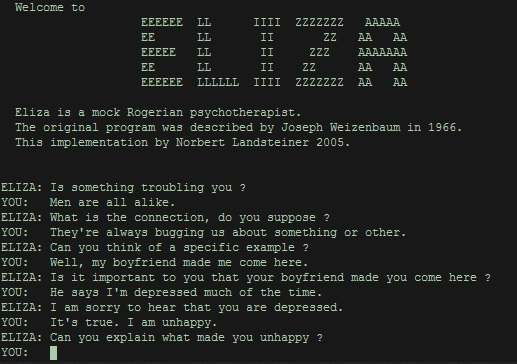
\includegraphics[width=0.7\linewidth]{part1/visuals/ELIZA_conversation.jpg}
    \caption{一段与 ELIZA 的典型对话}
    \label{fig:eliza}
\end{figure}

近年来，语言技术对社会的影响真正呈爆发式增长。我们每天都在与 ChatGPT、Claude 这样的聊天机器人打交道，可以用多种语言交流，增强型搜索引擎也已融入众多流行产品。然而，这些进展都建立在大量早期成果之上。一个著名的早期例子是 ELIZA——由 Joseph Weizenbaum 于 1966 年开发的心理治疗师聊天机器人 \citep{10.1145/365153.365168}。ELIZA 是一个简陋的聊天机器人，依靠简单的基于规则的词语替换（见图~\ref{fig:eliza}）。即便如此，它当时就已经被人们赋予了类人的特质。从这些基于规则的文本处理系统的早期岁月（那时我们依靠特定分隔符，比如空白，来切分词语），到今天，我们已经走了很远。 % to neural methods of language understanding. 
\begin{comment}
    
In this chapter, we will explore how language models actually generate responses to the text-based questions we pose, and how we might teach a machine to process languages that we humans use to communicate. 
First, in Section~\ref{sec:processinglanguage}, we will briefly discuss the basics of natural language processing. Then, in Section~\ref{sec:machinelearning} we will discuss machine learning aspects that are relevant for language learning and for agentic models. Finally, in Section~\ref{sec:modernNLP}, we will focus on modern deep learning approaches for language modeling, including transformers. 

\end{comment}




\subsection{语言理解与语言生成}
在考察计算机如何处理语言之前，我们先来看看人类是如何理解语言的。

一个关键观察是：交流是一个顺序过程，语言也因此被塑造成相应的形态。词语被一个一个地说出，也被一个一个地接收。这一规律对人类与机器处理语言同样成立：语言是字符的序列（阅读时）、音节的序列（说话时），或整个词的序列（在早期计算模型中）。

接下来，我们将深入考察为处理自然语言序列而发展出的技术。这些技术被划分为自然语言{\em 理解}与自然语言{\em 生成}两大类。下面我们分别简要介绍。

\begin{figure}
    \centering
    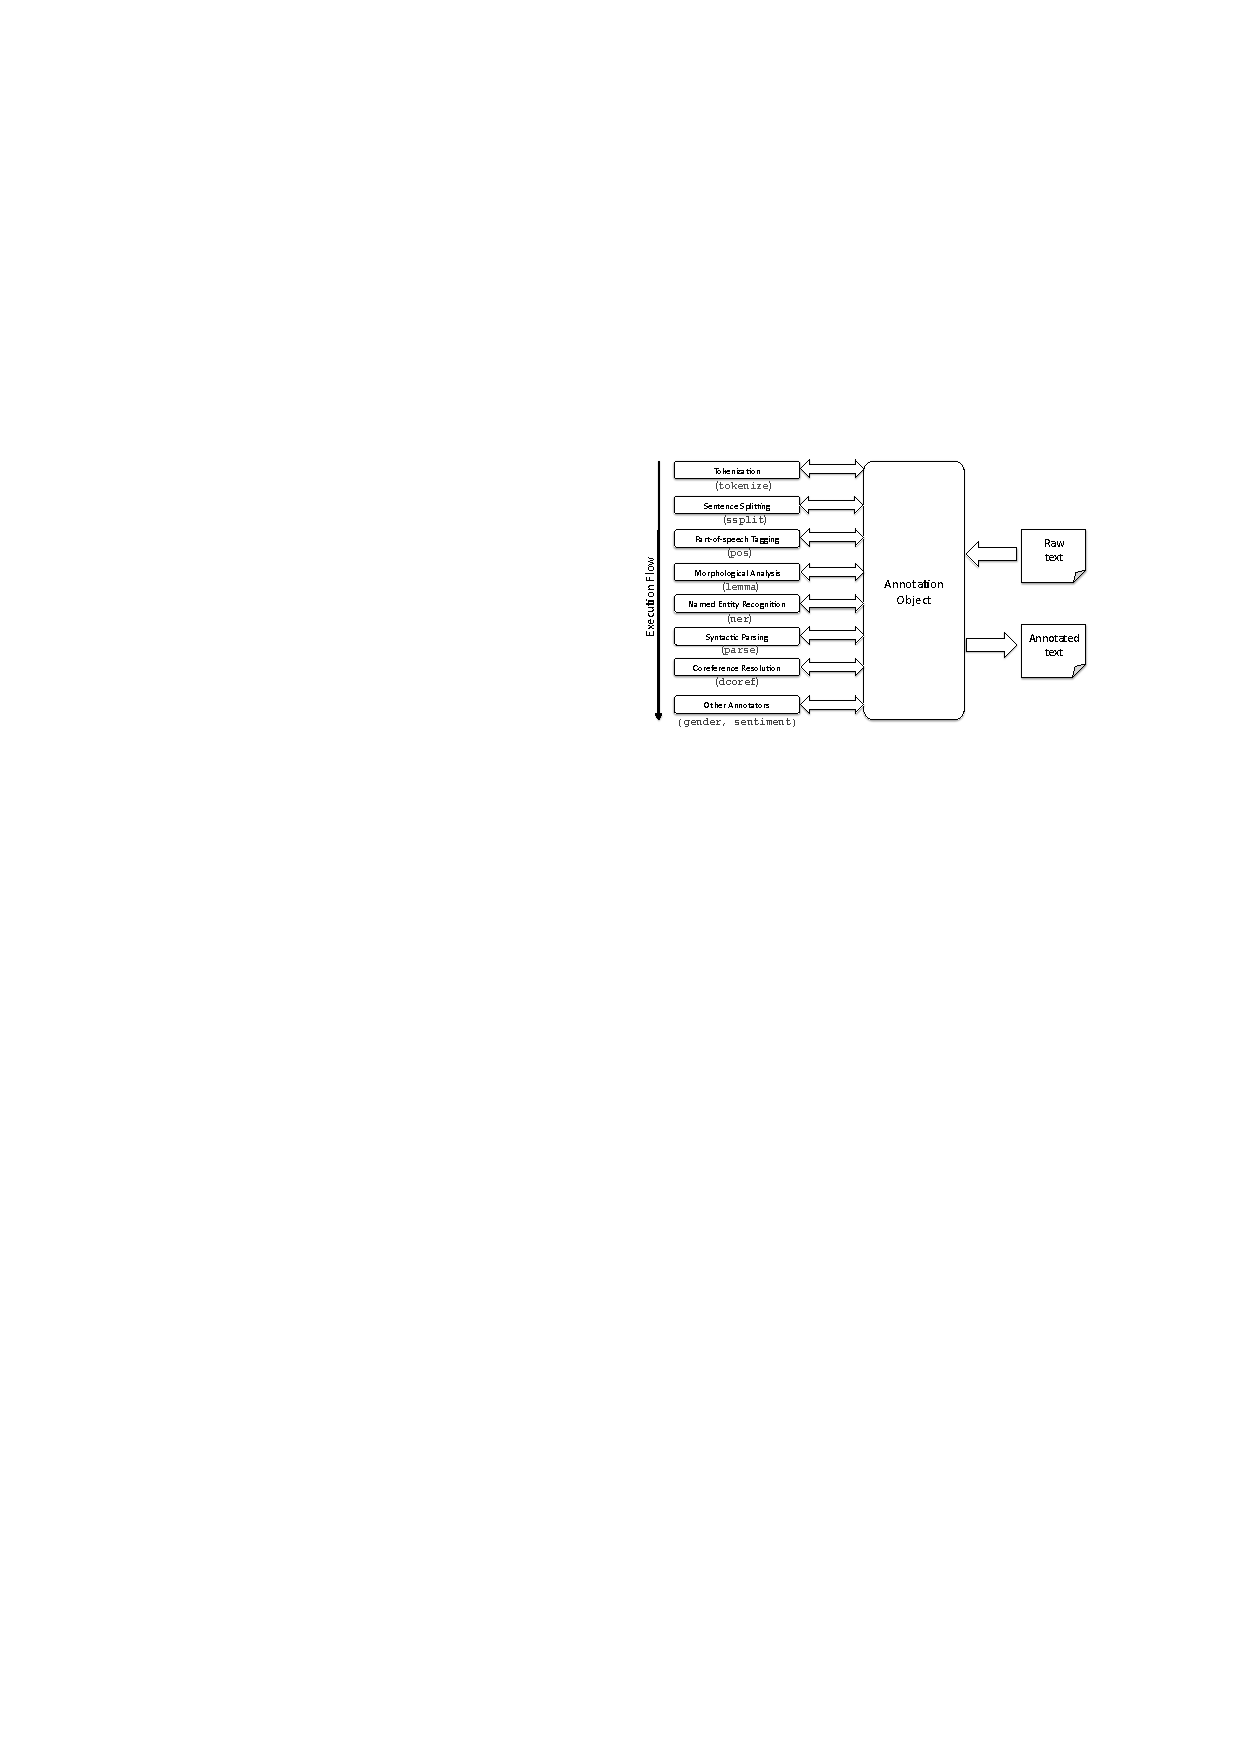
\includegraphics[width=0.66\linewidth]{part1/visuals/nlp_pipeline.pdf}
    \caption{标准的 NLP 流水线，由 \citet{manning-etal-2014-stanford} 绘制}
    \label{fig:nlp-pipeline}
\end{figure}

\paragraph{自然语言理解}
自然语言理解（NLU）致力于发展捕捉意义与意图的方法。NLU 的各种方法和技术把非结构化的人类语言要素映射为结构化格式，以便计算机能够解读并据此行动。这类技术可能包含若干处理层次，其思路受语言学分析启发（见图~\ref{fig:nlp-pipeline}），具体如下：
\begin{itemize}
\item 分词：确定有意义的语言单位（如词语）之间的边界，以供后续处理。
    \item 句法分析：确定语法结构（如主语、谓语、宾语）。
    \item 命名实体识别（NER）：识别并归类关键实体，如人名、日期与地点。
    \item 情感分析：检测一段文本的情绪基调。
    \item 共指消解：确定指称表达所指的人或物（例如：{\em 那台计算机}跟我说话）。
    \item 语篇分析：理解一个句子的含义如何受前文句子的影响。
\end{itemize}
%
%
NLU 面临的主要挑战之一是处理歧义 \citep{DBLP:conf/aaai/Roth98, liu-etal-2023-afraid}。人类语言中充满歧义，例如一词多义（同一个词有多种含义，如 {\em bank}），以及需要借助世界知识才能正确解读的语境依赖的细微差别。类似的挑战还有很多；自然产生的人类语言，其丰富与复杂程度恰如人类本身。

\paragraph{自然语言生成}
自然语言生成（NLG）致力于发展生成可读、自然的人类语言的方法。
其任务范围从自由形式的语言生成，到把结构化数据或模型表示转换为逼真的表述。

NLG 的一项重要任务是\emph{语言建模}（LM）。语言建模的任务是：给定前文语境，预测序列中的下一个元素。从数学上说，这相当于为词序列分配一个概率分布。传统上，求得这一分布依靠简单的基于计数的模型，这类模型往往还要借助进一步的简化假设，仅根据一个固定窗口的前文词来预测下一个词。

现代方法则使用精巧的神经方法，能够基于长上下文生成流畅的句子，这些句子在人类读者看来往往颇具意义。\footnote{而这本身并不总是难以做到，正如我们在 ELIZA 的例子中所见。}需要注意的是，有效的语言生成不仅仅要求语法正确，还要求连贯（逻辑顺畅）与衔接（语言上的联系）。当前的自然语言生成系统会使用采样方法、集成方法以及许多其他机制，在创造性与可预测性之间取得平衡，以确保输出读起来自然而不机械 \citep{li-jurafsky-2017-neural, 10.1145/3554727, gatt2018survey}。NLG 技术通常分为两类：
\begin{itemize}
    \item 抽取式生成：选取并重新组织已有的文本片段（常用于早期的摘要工具）。
    \item 生成式生成：从头生成全新的句子（如 ChatGPT 等现代模型所做的那样）。
\end{itemize}
大多数大语言模型采用生成式方法。

下面我们讨论语言建模的早期基础方法。我们先探讨语言的复杂性，再讨论分布式表示原理、分词方法以及早期的语言建模表示。

\subsection{自然语言的复杂性}
自然语言之所以难以被机器解读，原因有很多 %beyond those mentioned thus far 
。语言具有种种细微之处，它们或承载意义，或扭曲意义。要把握语言的全部微妙之处，仅理解其结构是不够的。此外，话语所处的语境也在交流中发挥作用。真正的理解要超越词语本身，去把握交流中蕴含的意图、言外之意与微妙之处 \citep{wittgenstein1953philosophical, Grice_1975, krause-vossen-2024-gricean-maxims}。下面我们介绍语言学领域研究的若干主题，每一个主题都从不同角度揭示语言能够表达什么。

\paragraph{句法} 句法规则支配句子的结构。在语言学研究中，句法指某一语言中规范句子结构的规则、原则与过程的总和。语言学的句法研究考察的是这样一种底层逻辑：它使说话者能够把词组合成合乎规范且有意义的序列。以英语为例，最常见的语序是主—谓—宾：在 {\em cat bites dog} 中，动词 {\em bites} 跟在主语 {\em cat} 之后，表明这句话的意思是「猫在咬」（而不是狗在咬）。
    
\paragraph{词法} 词法研究词如何根据其语法功能改变形态。词的形态变化与句法相关，而构词规则（及其例外）取决于具体语言（语系）。在上面那个例句中，动词 {\em to bite} 的形态变为 {\em bites}，其中的 {\em -s} 表示一般现在时（表示此事此刻正在发生，且施动者是单数，而不是古时候一群猫科动物所为）。
    
\paragraph{语义} 在语言学中，词汇语义学研究词的意义。在自然语言中，词的意义来源于它与其他词的关系。例如，意义几乎相同的词构成{\em 同义词}，如 car 与 automobile，或 vanish 与 disappear；意义相反的词构成{\em 反义词}，如 hot 与 cold，或 buy 与 sell。除此之外还存在许多其他关系。
    
在自然语言处理中，计算语义学研究的是如何在计算机中高效地表示这种意义。把句子存入计算机内存的一种基本做法，是直接用一组指向「该语言词表」的索引序列。然而，这种编码只记录了词是否出现，却没有记录词与词之间的关系；在这种朴素表示中，词的语义已不复存在。

词的意义来源于它与其他词的关系，因此我们需要一种能高效编码这些关系的方式。正如本章后文将会看到的，多年来人们发展出了多种解决方案，包括 Transformer 架构与注意力机制。
    
\paragraph{语用} 除了词的字面意义，人类还关心说话者的意图以及话语的语境。语言在特定社会语境中的使用方式决定了它的效果（{\em 意义即用法} \citep{baker2008wittgenstein}）。研究人类为保证交流有效而自然遵循的那些隐含的日常规则的学问，称为{\em 语用学}。

有一套奠基性的原则是格莱斯准则 \citep{Grice_1975}：人类用以推断意义的那些未言明的合作原则。例如，数量准则要求人们提供的信息恰好是对话所需的分量。这些准则塑造着我们的交流，使我们的语言变得可理解、可协作。对机器而言，要解读讽刺、言外之意或模糊指代（如「那个东西」），就需要掌握这些规则，而不能仅靠一本静态词典。

\paragraph{语篇} 语言很少以孤立句子的形式出现；它被组织成更大的单位，如段落、对话或完整文档。语篇研究关注句子如何相互连接，构成一个衔接且连贯的整体。机器要真正解读一段文本，就必须能够跨多个句子追踪实体，这项任务称为共指消解（例如，判断代词 {\em it} 指的是前一句中的猫、狗，还是「咬」这个动作）。理解语篇对于诸如文档摘要、机器翻译以及维持长对话等复杂的自然语言处理任务至关重要。

除上述主题外，还存在其他研究领域，如语音学（研究语言中承载额外交流含义的语音）、社会语言学（研究语言如何随阶层、地域等社会因素而变化）、词典编纂学（研究词典编纂的科学），以及许多其他领域。

正如以上概述所显示的，自然语言的生成与理解是庞大而艰难的领域。有一点很重要：语言并非静止不变。语言会随时间、地域、文化而变，也会随传播媒介而变 :-)。% \emoji{smiley}. 
正是这种变化，使语言技术的构建成为一项艰难且永无止境的探索。

在介绍那些至少能部分应对这些挑战的新技术之前，我们先讨论启发了自然语言处理现代转向的基本假设。

在计算机中表示自然语言之所以困难，是因为自然语言丰富而复杂。在本节余下的部分，我们将讨论分布式表示原理——它指出，一个词的语义由其周围的语境所决定。接着，我们会考察分词方法：把句子切分为词的方法。最后，我们将讨论如何借助词元向量得到一种能编码意义的表示。

\subsection{分布式表示} 
我们如何教会机器理解复杂的语义关系与语法结构，而不必把这一切都手工编码进去？答案在于分布式假设——现代自然语言处理的一块基石。其核心思想在 20 世纪 50 年代末被提出：
\begin{center}
    \emph{观其伴，知其义。（Firth, 1957）}
\end{center} 
%
这表明，一个词的意义可以从它通常出现的周围词（语境）中推断出来。出现在相似语境中的词，往往具有相似的意义。例如，如果 {\em coffee} 和 {\em tea} 都频繁出现在 {\em drink}、{\em sip}、{\em brew} 这类动词附近，机器就可以推断二者之间存在语义关联，而无需任何显式定义或人工提供的信息。

为了在计算上落实分布式假设，我们将借助线性代数，采用一种称为\emph{向量语义}的框架。我们把词表示为高维连续空间中的点。意义相近的词被映射到空间中彼此靠近的位置，而我们可用余弦相似度这类几何距离度量来衡量语义相似性（见图~\ref{fig:word-embeddings} 与第~\ref{sec:cosine} 节）。此外，我们还能通过向量运算来调整词义。
%
早期的实现依靠稀疏共现矩阵来构造语义向量，其做法是在语境中统计各个词的出现次数，与第 \ref{sec:early} 节所述的若干方法颇为相似。现代方法则倾向于使用稠密的低维向量，通常称为\emph{词嵌入}。这类表示一般通过训练神经模型来学习——让模型由邻近词预测某个词，或反过来，由某个词预测其邻近词。这一突破因 \emph{word2vec} 架构而广为人知 \citep{mikolov2013efficient}。


为词学习基于向量的表示，确实是捕捉意义的有效方式，但如果为语言中每一个独一无二的词都维持一个独立的向量，词表规模将大得不切实际。

此外，严格的词级方法难以处理罕见词或完全未见的词，因为模型对它们没有预先存在的向量。因此，在模型能为语言单位分配向量之前，我们必须先确定这些基本单位究竟是什么。为解决上述低效问题并处理未登录词输入，现代方法采用系统化的方式把原始文本拆解为更易处理的小块。这一过程称为分词，我们下面就来讨论。

\begin{figure}
    \centering
    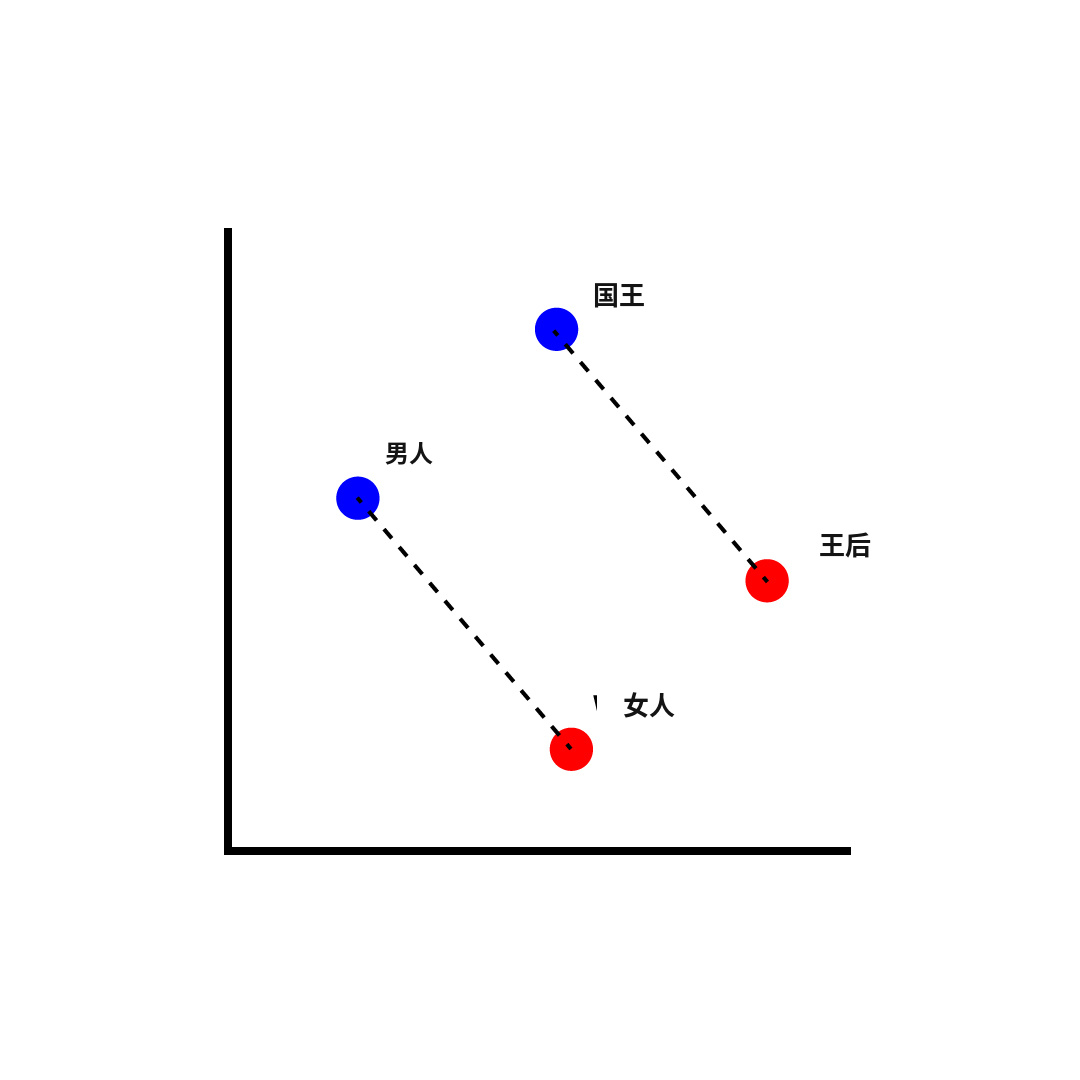
\includegraphics[width=0.66\linewidth]{part1/visuals/Word_vector_illustration.jpg}
    \caption{用 word2vec 嵌入进行向量运算的示意 \citep{singerep2022wordvector}。}
    \label{fig:word-embeddings}
\end{figure}

\subsection{分词}
\label{sec:tokenization}
在计算机能为语言赋予意义之前，它必须先有办法消化语言。假设我们手上已经有了原始文本——无论是从网上抓取的还是由语音转写的——那么当务之急就是确定如何把这些连续的字符串切分为有意义的单位，也就是如何把句子切分为词。这一过程称为\emph{分词}。然而，一个稳健的分词策略远不止按空格切分句子得到词那么简单；它还要能处理不同语言与方言的细微差异、解析复杂的标点，甚至要照顾到 emoji 这类现代产物，并把它们纳入一个大小固定的词表。

这一切分过程是许多自然语言处理流水线的关键一步。切分文本看似直截了当，但标点带来的歧义让这一过程变得复杂，例如缩写（N.L.P. 还是 NLP？）。简单的基于规则的分词器面对自然语言的结构不规则性，往往力不从心。因此，构造这些单位存在多种不同的做法，如例~\ref{ex:tokenization} 所示。

\begin{example}[分词策略]\label{ex:tokenization}
考虑下面这句话：\\ ``Leiden is beautiful in summer.''

\vspace{0.3cm}
\noindent\textbf{词级分词} \\
这种做法通常按空格和标点切分文本。\\
\vspace{0.1cm}
\noindent\texttt{["Leiden", "is", "beautiful", "in", "summer", "."]}

\vspace{0.4cm}
\noindent\textbf{字符级分词} \\
这种做法把文本拆解为单个字符。\\
\vspace{0.1cm}
\noindent\texttt{["L", "e", "i", "d", "e", "n", " ", "i", "s", " ", "b", "e", "a", "u", "t", "i", "f", "u", "l", " ", "i", "n", " ", "s", "u", "m", "m", "e", "r", "."]}

\vspace{0.4cm}
\noindent\textbf{子词分词（如 WordPiece）} \\
这种做法把常见词保留为完整词元，而把复杂或罕见的词拆解为基础子词。\\
\vspace{0.1cm}
\noindent\texttt{["Lei", "\#\#den", "is", "beautiful", "in", "summer",}\\ 
\noindent\texttt{"."]}
\end{example}

\paragraph{词级分词}
% \todo{Do we need references to the literature here?} -> Michiel: we don't, this is canon in NLP and there is no single paper/book for it (though we can go back to early linguistic works about the meaning of symbols).
这种做法把每个以空格分隔的字符串视为一个独立的词元。它保留了句法结构，却导致词表大得不切实际，并且受困于未登录词（OOV）问题——模型在训练中没见过的词上会失效。

大词表之所以成问题，原因在于\emph{独热编码}的机制。
% \todo{and here a ref?}  -> same reason as above
如果把词表 $V$ 中的每个词 $w$ 表示为一个向量 $\mathbf{x} \in \{0, 1\}^{|V|}$，其中只有对应 $w$ 的那一维为 1，那么维度 $|V|$ 就会随词表规模线性增长。由于这些独热向量之后要作为神经网络的输入，对于那些并不包含某个词表中全部词语的文本，我们最终会得到稀疏且计算低效的表示，而且无法捕捉词与词之间的语义关系。

\paragraph{字符级分词} 
纯粹的字符级建模看起来是应对词表膨胀问题的一剂良方，多年来也一直有人探索 \citep{mielke2021wordscharactersbriefhistory}。这种做法把文本切分为单个字符，从而把词表限制在字母表大小，几乎消除了未登录词问题。但它会显著拉长序列长度，由此带来的计算负担相当可观。此外，由于孤立的字符本身不携带语义，模型必须先学会词的形态，才能把握更宏观的语言模式，训练时间因而增加。

\paragraph{子词分词} 于是，目前大语言模型的标准做法在以上两者之间取得平衡：它把常见词保留为完整词元，同时把罕见词拆解为更小的、有意义的成分。代表性实现包括：

\begin{itemize}
    \item 字节对编码（BPE）：一种迭代算法，从单个字符出发，反复把最频繁的相邻词对合并为单个词元，直到达到目标词表规模 \citep{sennrich-etal-2016-neural}（例如 \textit{highest} $\rightarrow$ [\textit{high}, \textit{est}]）。BPE 最初是作为数据压缩算法提出的 \citep{gage1994new}。
    \item WordPiece：一种与 BPE 类似的迭代算法，但它依据似然准则而非原始频次来合并词对，目标是最大化训练数据的概率 \citep{wu2016googlesneuralmachinetranslation}。
\end{itemize}

\subsection{早期语言表示方法}
\label{sec:early}
分词之后，下一个问题是：如何把我们的语言单位（词元）组合成连贯且能承载意义的句子？我们从一个观察出发：在人类语言中，这些单位的排列顺序受严格的句法与语义规则支配。那么，如果我们计算方法能够准确地生成合理的文本序列，我们便可以说它具备了同样的句法与语义理解（至少是能够复现出这样的理解）。

我们如何构建能实现这一目标的数学表示？这项工作中的一项核心任务是\emph{语言建模}。从数学上讲，语言模型是一个函数，它计算一个词序列在特定语境中共同出现的联合概率。
通过计算这一概率，模型能够区分合乎逻辑、流畅的句子与随机的词元序列。例如在英语中，序列 \textit{the cat sat} 的概率显著高于 \textit{sat cat the}，因为前者符合既定的句法规则。

由于书面语言是顺序的，估计一个句子的联合概率本质上是一个序列估计问题。语言建模的总体目标，是根据句子由词 $w_1, \dots, w_k$ 构成的序列，量化给定句子 $S$ 出现在某一语言中的统计似然：

\begin{equation}
    \label{eq:language-sequence}
    P(S) = P(w_1, \dots, w_k)
\end{equation}

对于任意长度的句子，直接计算这个精确的联合概率在计算上是不可行的，因为任一给定词表中的词语组合数量呈指数级增长。为化解这一复杂性，我们通常借助概率的链式法则把联合概率分解开。通过对条件独立性作出特定的数学假设，这一分解能让计算在现实应用中保持可行 \citep{jm3}：

\begin{equation}
\label{eq:bigram}
    P(w_1, \dots, w_k) = P(w_1) \prod_{i=2}^{k} P(w_i \mid w_1, \dots, w_{i-1})
\end{equation}

通过最大化这一联合概率，概率模型学会偏向语法与逻辑上都站得住的序列。学到的概率分布实际上反向工程出了人类语言中那些复杂而未成文的规则 \citep{manning1999foundations}。要从切分好的文本语料中估计这些概率，早期方法依靠最大似然估计（MLE）。最简单的做法是根据一个词在语料中的相对频次来计算其边缘概率：

\begin{equation}
\label{eq:mle-word-prob}
    P(w) = \frac{\text{count}(w \text{ in corpus})}{\text{total number of words}}
\end{equation}

为让这些条件概率的计算变得可控，研究者借助\emph{$n$ 元模型}。一个 $n$ 元组是取自给定文本样本的 $n$ 个连续项构成的序列。与其计算一个词在其全部前文历史条件下的概率（这会很快变得计算上不可行），$n$ 元模型采用\emph{马尔可夫假设}。该假设认为，下一个词的概率只取决于它前面的 $n-1$ 个词，从而有效地截断了上下文。例如，二元模型（$n=2$）只通过紧邻的前一个词来近似历史。其条件概率的计算方式，是把两个词共同出现的频次除以第一个词单独出现的频次，

\begin{equation}
    P(w_i \mid w_1, \dots, w_{i-1}) \approx P(w_i \mid w_{i-1}) = \frac{\text{count}(w_{i-1}, w_i)}{\text{count}(w_{i-1})}
\end{equation}

同理，三元模型（$n=3$）以前两个词为条件。这种简化大幅降低了计算负担，使得直接从语料估计概率成为可能。

选取合适的 $n$ 涉及一个关键的权衡。$n$ 越大，能捕捉的上下文信息越丰富、句法依赖越深层，生成的模型语言也更自然。然而，增大 $n$ 会以指数方式加剧稀疏性问题：高度具体的词序列在训练数据中出现得少得多，模型将越来越频繁地遇到零概率。反过来，$n$ 越小，计数越稳健、越频繁，但会严重限制模型对更宏观语义以及句内长距离依赖的理解。

在标准的语言模型计算中，一旦遇到未见过的 $n$ 元组，概率就会变成零，而由于是连乘，这会让整个句子的联合概率一并归零。为缓解这种反直觉的行为，通常会对总计数进行平滑处理。一种常用技术是\emph{拉普拉斯（加一）平滑}，即给每一个可能的词表项都加上一个虚构的计数 $1$。为保持概率分布的有效性，分母要相应加上词表大小 $|V|$：

\begin{equation}
\label{eq:mle-word-prob-laplace}
    P_{\text{Laplace}}(w) = \frac{\text{count}(w \text{ in corpus}) + 1}{\text{total number of words} + |V|}
\end{equation}

这些基于概率与计数的方法最终给出了语言的数值表示。一个好的表示应当编码出我们凭直觉就能把握的词的属性：它的意义、它的语法功能，以及它与其他词的关系。在早期自然语言处理中，这些相对频次与共现计数被组织成向量，依据词在文本中的分布来表示词。

基于计数的表示虽然可行，但得到的向量维度高、稀疏，导致计算低效，且对未见数据泛化不佳。因此，现代自然语言处理已转向用神经网络学习稠密的低维向量表示，即\emph{嵌入}。这类模型不再依赖显式计数，而是在「由周围语境预测某个词」这一任务的副产品中学习连续表示，从而以更高效的形式捕捉更深层的语义关系。
这些现代方法将在第~\ref{sec:modernNLP} 节讨论。在此之前，我们先插入一段简要的过渡，回顾三种重要的机器学习方法。

\section{面向自然语言处理的机器学习方法}
\label{sec:machinelearning}
\chaptermark{面向 NLP 的机器学习方法}
在建立了语言表示的入门知识后，我们现在转向学习算法——正是它们让我们得以构建驱动现代人工智能系统的大模型。大语言模型是用机器学习这一更广阔领域中的方法来训练的。机器学习是一个庞大的研究领域，但理解大语言模型只需熟悉三种核心范式及其在语言建模中的用法：\emph{监督学习}、\emph{自回归学习}与\emph{强化学习}。我们简要涉及这些基本方法，更深入的探讨请参阅标准著作。

\subsection{监督学习} 
监督学习是机器学习的基石。它之所以叫「监督」，是因为它依赖一组必须事先给定的标签，由这些标签来\textit{监督}训练过程。这种做法使用一个由「样本—标签」对构成的数据集 $D = \{(x_i, y_i)\}$，来训练预测模型 $f_\theta$ 的参数 $\theta$。该模型可用于为每个输入 $x$ 计算一个估计值 $\hat{y}$，数学上记作 $f_\theta(x) \rightarrow \hat{y}$。用模型计算这一估计值的过程也称为{\em 推理}，或{\em 前向传播}。

前向传播之后，我们可以用损失函数 $\mathcal{L}$ 来计算估计值 $\hat{y}$ 与真实标签 $y$ 之间的某种差异。常见的损失函数有统计回归中的平方差损失 $\mathcal{L} = \sum_i(\hat{y_i} - y_i)^2$，以及分类中的交叉熵损失 $\mathcal{L} = -\sum_cy_c\log(\hat{y_c})$。
 
监督式训练算法的目标，是通过调整参数，使数据集上所有样本对的损失之和最小。这一步在{\em 反向传播}中完成。在这里，损失函数被用来计算误差信号，据此调整模型 $f$ 的参数 $\theta$，使下一次前向传播能得到更低的损失（误差的反向传播）。在数据集样本上最小化损失函数的过程称为\emph{训练}。对全部训练数据完整地做一遍前向与反向传播，称为一个\textit{轮次}（epoch）（出于效率考虑，一个轮次可以拆分为若干训练\textit{批次}）。

训练完成后，为了检验模型 $f_\theta$ 是否好用——即能否泛化到未见过的样本——我们要用不属于训练集的新样本对它进行\textit{测试}。

如果模型在训练集上的准确率高，我们说它训练得好（训练收敛）。如果它在测试集上的准确率也高，我们就说它泛化得好，训练目标达成。通俗地说，如果模型在训练集上准确率高、在测试集上却低，我们就说模型在训练集上过拟合了。这通常意味着模型训练过久或参数过多，以致它不仅学到了训练集中的信号，也学到了噪声。如果模型在训练集和测试集上准确率都低，我们说它欠拟合。这多半是因为训练太短，或者模型太简单（可训练参数太少），不足以刻画数据的复杂性。

一般来说，变量少的问题（低维问题，如简单回归）只需要较小的模型（更少的参数）和较少的训练数据就能表现良好。变量多的问题（高维问题，如图像分类）则需要拥有数百万参数的大模型（往往是深度神经网络）以及大规模训练数据集才能表现良好。事实上，图像分类的突破性表现 \citep{krizhevsky2012imagenet} 正是在构建了包含数百万张人工标注图像的大规模数据集 ImageNet 之后才取得的 \citep{deng2009imagenet}。

监督学习是机器学习的根基。关于这一主题已有许多优秀教材 \citep{bishop2023deep,goodfellow2016deep}。它也是大语言模型训练的核心技术之一，例如监督微调，我们将在下一章看到。

\subsection{自回归学习} 
大语言模型是以自回归方式训练的。在这种训练方式中，并不存在由带标签样本对构成的数据集，但可用的（文本）数据非常丰富。自回归学习是一种自监督学习，不需要显式标签，而是利用数据固有的顺序性来预测下一个词元。

在语言模型的自回归预训练中，我们的算法在数据集上进行预测：每个词元 $y=x_t$ 都被当作其前面若干示例词元 $\mathbf{x}=x_{t-1}$ 的标签。自回归学习是现代自然语言处理的一项核心任务，既被用于当代的模型训练流水线 \citep{radford2018improving}，也被写入自然语言处理教材 \citep{jm3}。关于这些方法的更多细节，我们将在第~\ref{sec:modernNLP} 节与第~\ref{chap:pipeline} 章中给出。

\subsection{强化学习} 
\label{sec:sdp}\label{sec:rl}
监督学习和自回归学习都需要一个训练数据集——它们是在已有数据上{\em 离线}训练的。然而有时并没有现成的数据集，但我们可能拥有一个函数，它能告诉我们当前处于好状态还是坏状态。这时就可以使用一种称为强化学习（RL）的{\em 在线}学习方法：智能体执行动作 $a$，把环境从状态 $s$ 带到下一个状态 $s'$，随后环境回报该新状态的奖励 $r(s')$。（之所以称为在线，是因为它在训练过程中即时生成自己的训练数据。）智能体随后可以利用这些奖励信息，调整一个由 $\theta$ 参数化的行为策略函数 $\pi_\theta(s) \rightarrow a$，从而知道在哪个状态下该执行哪个动作。当所面对的问题是顺序决策问题时，动作 $a$ 把系统从状态 $s$ 带到另一个状态 $s'$，而奖励取决于过去所采取的动作（这就是信用分配问题：奖励应当归给哪些动作？）。重复「状态／动作／奖励」这一过程，可以让智能体探索整个状态空间，并学得一个对所有权状态都适用的最优策略 $\pi^*(s)$。%, solving the credit assignment problem.  

\begin{figure}[tb]
  \begin{center}
    \input figures/rl
    \caption{强化学习，据 \citet{sutton2018reinforcement}}\label{fig:rl-org}
  \end{center}
\end{figure}

注意，强化学习是在线的，因而本质上带有循环性。开始时，策略 $\pi$ 见过的奖励很少，只在少数几个状态上拥有「该采取哪个动作」的有用信息。如果它贪心地直接利用这些信息，就只会遍历环境中很有限的一部分，找到的最优策略也只是局部最优。为找到更好的最优解，它应当探索，尝试随机动作，最好能覆盖整个状态空间。

强化学习是一种主动的智能体式学习，其信号来自环境的反馈。一个关键观察是：判断一个输出好不好（奖励函数）通常比从零造出一个新输出（带标签数据集）更容易。
人们已经发展出许多专注于良好探索方法的强化学习算法。
强化学习问题被形式化为马尔可夫决策过程（MDP），它由状态表示 $S$、动作函数 $A(s)$、转移函数 $T(s, a) \rightarrow s'$ 以及奖励函数 $R(s)$ 构成。奖励是环境给出的、对状态优劣的数值指示，可正可负。智能体的目标是找出在每个状态 $s$ 下采取最优动作 $a*$ 的策略 $\pi(s)$。
图~\ref{fig:rl-org} 展示了强化学习智能体如何通过与环境的交互，在线学得一个为每个状态指定动作的策略；环境能够计算函数 $T$ 与 $R$（环境会回答智能体的提问：它这个动作导致的下一个状态是什么，那个状态有多好）。

当状态空间小到能放进计算机内存时，我们可以使用精确的表格型强化学习方法，如 Q 学习 \citep{watkins1992q}。对于更大的问题，则使用函数逼近方法（深度神经网络），如深度 Q 学习（DQN）\citep{mnih2015human} 或近端策略优化（PPO）\citep{schulman2017proximal}。在深度强化学习中，策略是一个参数化的神经网络，像监督式深度学习那样通过反向传播来训练。

强化学习是现代推理型语言模型的基础。关于强化学习已有许多教材，例如 \citet{sutton2018reinforcement} 的开创性著作，以及若干更具教学性质的读物 \citep{graesser2019foundations,plaat2020learning,plaat2022deep}。在大语言模型训练中，强化学习被用于强化微调与多步推理，我们将在第~\ref{chap:reasoning} 章看到。此外，强化学习把机器学习问题表述为「智能体试图学会如何在环境中交互」，这恰好契合智能体式大语言模型的设定。在智能体式大语言模型中，它被用于提示词优化的上下文强化学习、世界模型，以及为其他智能体相对于环境的行为建模，我们将在本书后文看到。


强化学习之所以是一种受欢迎的机器学习方法，是因为我们可以在没有现成数据的新环境中学习——方法自己生成数据。 %New environments can be explored for which no dataset exists yet. 
在考虑使用强化学习时，应当回答两个问题：（1）当前问题是否为顺序决策问题；若是，（2）状态空间有多大——我们可以使用精确的表格型方法，还是必须求助于函数逼近？

%Going from state to next state allows sequential decision problems to be solved, where choices in the past determine the outcome in the future. For this, the credit of a certain state must also be assigned to previous states, so that we know the right action in all states. Reinforcement learning is an open and flexible paradigm, powerful, when caveats of exploration and credit assignment are taken care of.


既然我们已经讨论了必要的语言与机器学习原理，现在回到语言本身，进入下一步：对语言建模。  

\section{为语言建模}\label{sec:modernNLP}
在语言表示与机器学习的基础知识之后，我们转向用于构建计算语言建模能力的几种总体范式。自然语言处理的发展大致可由三种范式来刻画。每一种范式都代表着「用什么类型的模型来把握语言」以及「如何应对人类语言固有复杂性」这两点上的一次根本转变。我们将看到，随着范式更替，我们引入了越来越多的机器学习技术，利用算力的增长来处理更多数据，以训练出越来越大的神经网络来完成语言处理。这三种范式是\textit{符号式}、\textit{统计式}与\textit{神经式}方法 \citep{kautz2020third, deng2018deep}。
% \todo{Hebben we een ref voor dit mooie historische overzicht?}  -> toegevoegd, de tweede citatie noemt het "rational" "empirical" en "deep learning" maar dat vind ik maar vaag

\paragraph{符号式方法} 这类方法常被称为\textit{经典人工智能}或基于规则的系统；它们与早期的 ELIZA 一样，依赖明确的人工定义指令。符号式模型把语言视为一个形式系统，试图以演绎方式解析意义。这类系统在设计上高度透明、可解释，但很脆弱：它们用僵硬的规则（\textit{if-then-else}）去应对现实语言中的自然变异、习语表达与歧义时，往往力不从心。要把符号式方法扩展到更大的语言任务，就需要人工穷举大量边缘情况，这种劳动密集的做法在除最小问题领域之外都不可行。

\paragraph{统计式方法} 为克服僵化规则集的局限，1980 至 1990 年间，该领域经历了一次走向概率建模的实证转向。统计式方法不再依赖显式的句法规则，而是利用大规模文本语料来计算词共现的可能性，例如隐马尔可夫模型与 $n$ 元语言模型。这种数据驱动的方法扩展性好，处理语言歧义与噪声的能力远胜于此前的符号式方法。然而，由于这类模型通常依赖马尔可夫假设， %\footnote{The Markov property describes a memoryless, stochastic process, where future states depend only on the current state, not on past states (or, to put it differently, relevant history must be encoded in the current state). It simplifies complex systems reasoning, and allows efficient algorithmic and mathematical reasoning. The Markov property may be an oversimplification, especially in language, where elements far far away---not encoded in the previous word---may influence current meaning.} 
它们对意义的表示本质上局限于局部的词语模式，因而难以捕捉长距离依赖与更宏观的语境。

\paragraph{神经式方法} 大约在 2010 年之后，当代的最先进技术转向了神经网络与深度学习。神经式方法不再使用逻辑或离散计数，而是把语言单位表示为连续语义空间中的稠密低维向量。现代架构——尤其是 Transformer——采用注意力机制，同时在整个序列上建模全局语境。这种做法带来了令人印象深刻的泛化能力、流畅的文本生成以及跨语言能力。不过，这些优势也伴随显著的取舍：神经模型在很大程度上是黑箱，牺牲了符号式方法那种可解释性，而且需要大规模数据集与大量计算资源。

当代的自然语言处理训练流水线从上述三种范式中都汲取了灵感。在下一章描述一个示例流水线之前，我们需要更深入地理解这些组成部分的核心构件，因为它们是智能体式大语言模型所依托的系统的基本模块。在接下来的几节中，我们将讨论许多主题：词嵌入、语境化嵌入、序列建模、注意力、Transformer、编码器（如 BERT）以及解码器（如 GPT）。  

\subsection{嵌入}\label{sec:cosine}
早期的神经嵌入模型通过定义上下文窗口来落实词汇项的语义理解：即以目标词为中心、左右各 $n$ 个词的跨度，并预测缺失的中心词。对于句子 \textit{There are two cookies left on the table}，若设窗口为 $n=2$，则 \textit{cookies} 的上下文词是 \textit{are}、\textit{two}、\textit{left} 和 \textit{on}。把这个窗口系统地在大型文本语料上滑动，我们就能统计每个词出现在其他每个词的上下文中的次数。这些计数构成共现矩阵的基础：每一行代表一个目标词，每一列代表一个上下文词，单元格中的数值就是列词出现在行词上下文中的次数。例如，\textit{cherry} 的向量在 pie 那一列上可能有很高的值（比如 442），而在 computer 那一列上很低（比如 2）。\textit{strawberry} 的向量会呈现类似的模式，从而反映出这两个词之间的语义相似性。

通过把词表示为向量，我们把它们置于一个高维向量空间中，其中每一维对应一个上下文词。在这个空间里，意义相近、共享相似上下文的词会指向相近的方向。这种几何关系使我们能够用数值来衡量语义相似性。最常用的方法是\emph{余弦相似度}，它衡量两个向量 $\mathbf{a}$ 与 $\mathbf{b}$ 之间夹角 $\theta$ 的余弦，如式~\ref{eq:cosine} 所示。

\begin{equation}
    \label{eq:cosine}
\text{similarity} = \cos(\theta) = \frac{\mathbf{a} \cdot \mathbf{b}}{\|\mathbf{a}\| \|\mathbf{b}\|} = \frac{\sum_{i=1}^{n} a_i b_i}{\sqrt{\sum_{i=1}^{n} a_i^2} \sqrt{\sum_{i=1}^{n} b_i^2}}
\end{equation}


前面我们说过，基于计数的向量会导致维度随词表规模线性增长的高维空间。由于维度数量决定了后续模型的计算复杂度，我们希望把维度控制在合理范围，转而构造稠密的嵌入。为此，我们使用经典的 word2vec 算法 \citep{mikolov2013efficient}。这种做法先随机初始化一个嵌入矩阵 $W$，再迭代更新它，使之符合「相似的词出现在相似的上下文中」这一直觉。这一总体框架采用两种不同的技术来实现该目标：skip-gram 与连续词袋，如图~\ref{fig:word2vec} 所示。

第一种是 \emph{skip-gram}，它预测给定目标词周围可能出现哪些上下文词。它更新矩阵，使正样本（真实的目标—上下文词对）之间的余弦相似度尽可能高，同时压低负样本（随机配对的词）的相似度。由于 skip-gram 把每一个「目标—上下文」配对都视为一条独立的训练观测，即使对不常见的词，它也会对错误预测施以重罚。因此，skip-gram 擅长捕捉细粒度的语义细节，即使对罕见词也能给出准确的表示。

第二种是\emph{连续词袋}（CBOW），它执行的是相反的操作：根据周围上下文词的组合来预测单个目标词。由于在预测目标词之前先对上下文向量取了平均，CBOW 本身就抹平了各个上下文词的细节。这种分布式的平滑正是它性能特点迥异的原因：CBOW 的训练速度显著快于 skip-gram，在捕捉高频词之间的一般句法关系上非常有效，但对罕见词的敏感度有所牺牲。

\begin{figure}[tb]
    \centering
    \begin{minipage}{0.45\textwidth}
        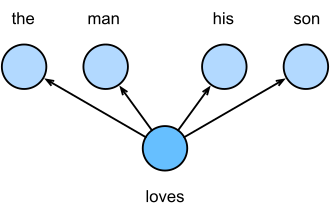
\includegraphics[width=\textwidth]{part1/visuals/skipgram.png}
    \end{minipage}
    \hfill
    \begin{minipage}{0.45\textwidth}
        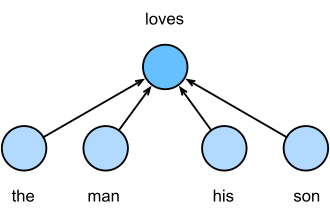
\includegraphics[width=\textwidth]{part1/visuals/cbow.png}
    \end{minipage}
    \caption{构造词嵌入的 skip-gram（左）与连续词袋（右）方法示意 \citep{d2l_cbow_2023}。}
    \label{fig:word2vec}
\end{figure}



\subsection{转向语境化嵌入}
word2vec 在构建高质量词嵌入方面是一次重大飞跃。然而它有一个主要缺点：word2vec 产生的是\textit{静态嵌入}。这意味着无论一个词如何使用（处于什么语境），它都被映射到同一个向量。这就在一词多义上造成了根本性的问题。考虑 \textit{bank} 一词在两个不同句子中的用法：
\begin{enumerate}
    \item I need to go to the \textit{bank} to withdraw some money.
    \item The swimmer sat on the river \textit{bank}.
\end{enumerate}
在静态模型中，\textit{bank} 只有一个固定表示，它必须在这两种迥异的含义之间取平均或做出取舍，结果得到一个既不纯粹是金融、也不纯粹是地理，或者两者怪异地混杂在一起的向量。现代架构（如本章后文讨论的 BERT 与 GPT）通过产生\textit{语境化嵌入}来解决这个问题。模型不再查一张静态的查找表，而是处理整个序列；\textit{bank} 得到的向量依据周围词元（\textit{money}、\textit{withdraw} 对 \textit{river}、\textit{swimmer}）动态计算，从而使机器能够表示说话者想要表达的具体含义。


\subsection{循环神经网络}
嵌入能够表达单个词的复杂语义，但我们仍然需要一种高效的方式把语言作为序列来摄入。例如，训练分类任务模型时，需要引入独立性假设来简化计算上的依赖关系。我们也可以采用滑动窗口的做法，把相关的词嵌入拼接成一个向量来表示句子。然而这会迅速增大任何分类器的输入规模，并且无法扩展到长文本序列。

对人类而言，我们对下一个观察对象的预期，取决于过去见过（或听过）的东西。此前，模型通过独立性假设来近似这一直觉，如式~\ref{eq:bigram} 所示。形式上，我们为按序列 $x_1, x_2, \dots, x_t$ 出现的输入 $x$ 引入额外的记号，时间步从 1 到 $t$。在这一表述下，预测下一个词可以建模为 $P(x_{t+1} \mid x_1, \dots, x_t)$。或者，我们把 $x_{t+1}$ 称为时间步 $t$ 的预测 $y_{t}$。 
% our models produce output predictions for corresponding timesteps $y_1, \dots, y_t$. 

要按序列有效地观察输入并给出相应预测，我们必须把历史语境纳入模型。这意味着，除了当前输入之外，我们还要纳入模型此前的隐藏状态。\emph{循环神经网络}（RNN）就是带有这种循环的网络：其当前取值既取决于输入，也取决于网络在上一时间步的状态。我们不再只产生一个预测（例如一个词或词元）$y_t$，而是同时维护一个隐藏状态 $h_t$。形式上，这由式~\ref{eq:rnn_h} 与式~\ref{eq:rnn_y} 表达。图~\ref{fig:rnn} 展示了 RNN 的架构，以及我们如何想象它在时间步上的展开。
%
\begin{figure}[tb]
    \centering
    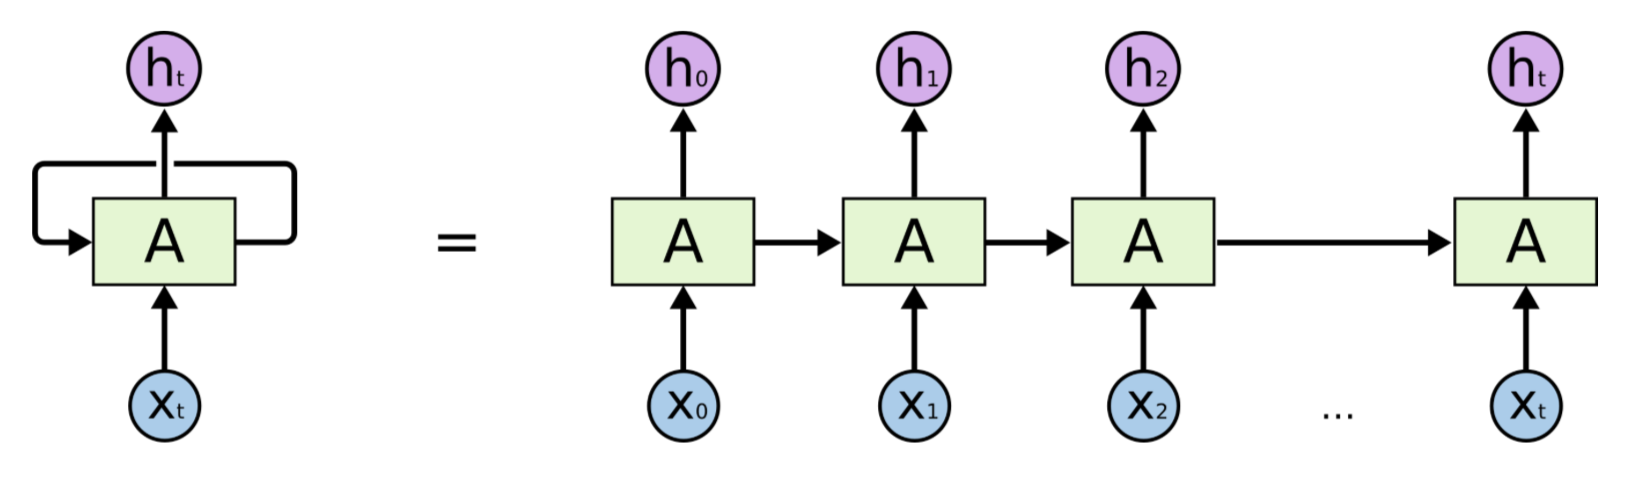
\includegraphics[width=\linewidth]{figures/RNNcolah.png}
    \caption{展开的 RNN（插图来自 Chris Olah 的博客 \citep{olah2015understanding}）}
    \label{fig:rnn}
\end{figure}
%
\begin{align}
    \label{eq:rnn_h}
    h_t &= f(\mathbf{U}h_{t-1} + \mathbf{W}x_t + \mathbf{b_h})\\
    \label{eq:rnn_y}
    y_t &= g(\mathbf{V}h_t + \mathbf{b_y})
\end{align}
%
这引入了新的可训练参数矩阵 $\mathbf{U}, \mathbf{V}, \mathbf{W}$（以及相应的偏置项 $\mathbf{b}$），以确保我们的架构能够相应地塑造隐藏状态与输出 logits。RNN 理论上可以处理无限长的序列，我们也不再需要马尔可夫假设来应对稀疏性问题。

RNN 的训练使用时间反向传播（BPTT）：我们把时间上的依赖关系展开，从而把梯度从时间步 $t$ 反向传播到更早的时间步：$t_{-1}, t_{-2}, \dots$。然而，由于在某一时间步更新模型所用的梯度递归地依赖此前各时间步，这一步是敏感的。又因为链式法则要求反复做矩阵乘法，这就导致了\emph{梯度消失或爆炸}问题 \citep{bengio1994learning, pmlr-v28-pascanu13}。在 RNN 中控制信息流动是困难的：与较新的信息相比，来自早期时间步的信息对梯度的影响相对很小。在实践中，用 RNN 学出显著信号往往是件难事。

\begin{figure}[tb]
    \centering
    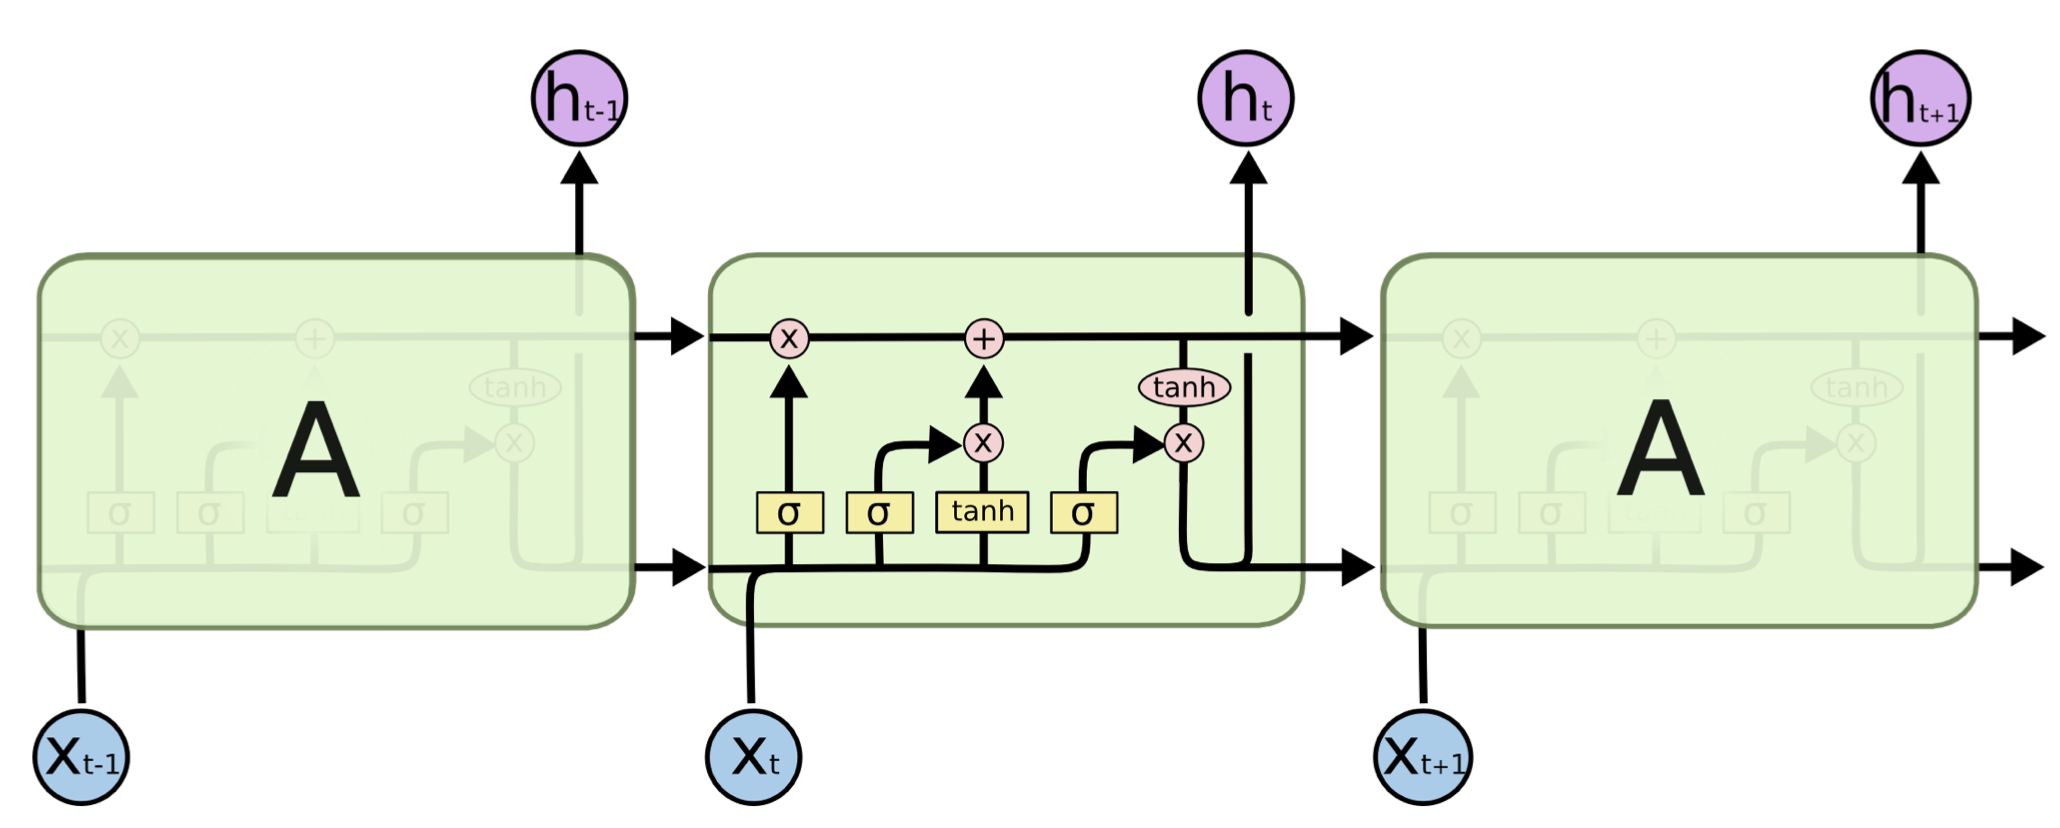
\includegraphics[width=\linewidth]{figures/LSTMcolah.png}
    \caption{LSTM 的重复模块（插图来自 Chris Olah 的博客 \citep{olah2015understanding}）}
    \label{fig:lstm}
\end{figure}

\paragraph{LSTM} \emph{长短期记忆}（LSTM）架构是为解决梯度问题而提出的 \citep{hochreiter1997long}。LSTM 通过控制信息流动来工作。在 LSTM 网络中，人们添加了额外的门来构造一个上下文向量，网络将学会向其中添加和更新信息（见图~\ref{fig:lstm}）。下面是 LSTM 架构在单个时间步 $t$ 上的数学定义。LSTM 维护两个状态：上下文状态（$c_t$）与隐藏状态（$h_t$），并用门来控制信息流动：
\begin{align*}
    f_t &= \sigma(U_f h_{t-1} + W_f x_t) \\
    k_t &= c_{t-1} \odot f_t \\
    g_t &= \tanh(U_g h_{t-1} + W_g x_t) \\
    i_t &= \sigma(U_i h_{t-1} + W_i x_t) \\
    j_t &= g_t \odot i_t \\
    c_t &= j_t + k_t \\
    o_t &= \sigma(U_o h_{t-1} + W_o x_t) \\
    h_t &= o_t \odot \tanh(c_t)
\end{align*}
%
在上面的记号中，$\odot$ 表示两个向量的逐元素相乘，也称为哈达玛积。除 LSTM 之外，还有若干后续变体，例如\emph{门控循环单元}（GRU），它在计算复杂度与可训练参数数量之间取得平衡 \citep{cho2014gated}。

循环神经网络在语言建模中扮演过重要角色。关于 RNN、LSTM 与 GRU 如何工作的进一步解释，可参见 \citet{olah2015understanding,bishop2023deep,goodfellow2014generative}。

% maybe not so relevant
% The GRU merges the cell and hidden states into a single state ($h_t$), and also uses a series of gates. 
% \begin{align*}
%     z_t &= \sigma(U_z h_{t-1} + W_z x_t) \\
%     r_t &= \sigma(U_r h_{t-1} + W_r x_t) \\
%     g_t &= \tanh(U_g (r_t \odot h_{t-1}) + W_g x_t) \\
%     h_t &= (1 - z_t) \odot h_{t-1} + z_t \odot g_t
% \end{align*}

\paragraph{编码器—解码器}
到目前为止，我们把任务表述为语言建模任务：给定前文语境，如何预测下一个词。然而，还有另一种任务表述值得介绍。

考虑机器翻译问题。它看起来与前面「根据输入 $x_1, \dots, x_t$ 预测词元 $x_{t+1}$」的任务相似，但我们现在面对的是一个\emph{序列到序列}（seq2seq）问题：我们需要处理一种语言中的输入句子 $x_1, \dots, x_n$，并输出另一种语言中的译文句子 $y_1, \dots, y_m$。为什么翻译是一个 seq2seq 问题？请注意 $n$ 与 $m$ 可以彼此不同，而且译文未必保持原来的顺序，如下面这个英译荷的例子：
\begin{center}
    \emph{We will celebrate the relief of Leiden} (7 words)\\[.5em]
    \emph{Wij gaan Leids Ontzet vieren} (5 words)
\end{center}
%
\emph{编码器—解码器}架构是一个强大的框架，专门用来处理输入与输出长度可能不同的序列到序列任务。编码器与解码器是两个各自独立的 RNN，它们协同工作，把变长输入映射为变长输出。编码器的任务是逐步处理输入序列，并把信息压缩成一个固定长度的向量，通常称为上下文向量。\footnote{不要与 LSTM 的上下文向量混淆。自然语言处理研究在很短时间内就重新使用了这一术语。研究论文中的语言也是一个移动的目标。}这就把信息挤进了一个\emph{瓶颈}：把输入序列 $x_1, \dots, x_t$ 的信息压缩成单个隐藏向量。然而这一过程难以建模，且会损失信息。该架构的示意见图~\ref{fig:encdec}。

\begin{figure}
    \centering
    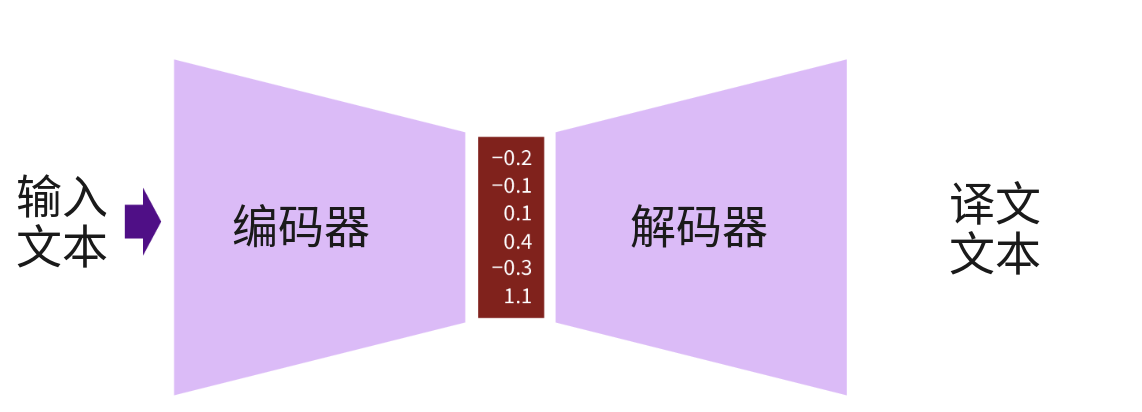
\includegraphics[width=0.65\linewidth]{figures/encdec.png}
    \caption{编码器—解码器架构示意}
    \label{fig:encdec}
\end{figure}

上下文向量充当编码器与解码器之间的桥梁。它是编码器的最后一个隐藏状态，被作为初始隐藏状态传给解码器。这个向量编码了整个源句子的语义，使解码器能够开始准确地生成目标序列。解码器是第二个 RNN，它以该上下文向量为条件产生输出词元，目标是逐个词元地生成输出序列，直到生成一个特殊的序列结束词元为止。这种做法在原理上是可行的。然而，把一句很长的输入硬塞进单个固定长度的上下文向量会造成信息损失（瓶颈问题）。此外，RNN 在读到长序列末尾时，往往记不住开头的内容。这两个问题叠加，促使人们去发展更动态的信息传递方式，我们下面就来讨论。




\subsection{注意力}
为了寻找瓶颈问题的解法，研究者设法把整个序列各处的信息高效地传入解码器。这样在生成过程中，解码器就能判断输入序列的哪些部分与解码下一个词相关。

这一探索催生了各种先进的注意力机制 \citep{DBLP:journals/corr/BahdanauCB14,kim2017structured}。%These attention mechanisms aim to address this problem. 
注意力机制的效果见图~\ref{fig:enc-dec-bleu}，图中绘出了翻译性能（以 BLEU 分数衡量 \citep{papineni2002bleu}，越高越好）。采用注意力机制的架构（称为 \textit{RNNsearch}，见图~\ref{fig:enc-dec-bleu}）始终能够取得较高的翻译质量，尤其是在长句上。而标准的 RNN 编码器—解码器模型（\textit{RNNenc}）则随句子变长而性能急剧下降。

\begin{figure}[tb]
    \centering
    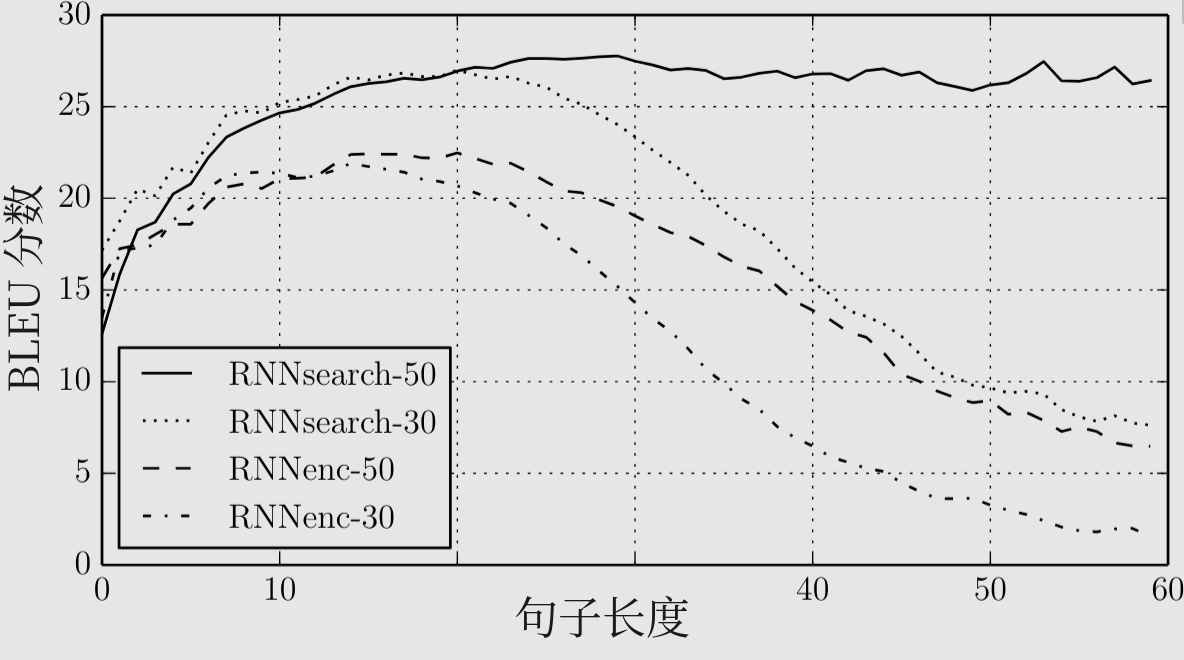
\includegraphics[width=0.66\linewidth]{part1/visuals/enc_dec.png}
    \caption{生成译文相对于句子长度的双语评估替补（BLEU）分数 \citep{DBLP:journals/corr/BahdanauCB14}}
    \label{fig:enc-dec-bleu}
\end{figure}


注意力背后的直觉是：在上下文向量中纳入所有编码器隐藏状态的线性组合，而不是只依赖最后一个隐藏状态。这使模型能够回头关注输入序列中与当前正在生成的词相关的特定部分。我们可以通过调整线性组合中每个输入词元 $x_i$ 的权重 $a_i$，来控制它受到的关注程度，如式~\ref{eq:enc-dec-attention} 所示。这里 $\mathbf{c}_j$ 是第 $j$ 个输出对应的上下文向量，$h_i$ 表示第 $i$ 个输入词元的隐藏状态。

\begin{equation}
\label{eq:enc-dec-attention}
    \mathbf{c}_{j} = a_1\mathbf{h}_1, \dots, a_n\mathbf{h}_n
\end{equation}

权重 $a$（常称为注意力权重）并非固定不变，而是动态计算出来的。一个关键观察是：我们可以利用隐藏状态 $h_i$——它是词元或词语义的表示。通过比较两个隐藏状态，例如计算它们的余弦相似度，我们就能判断其中一个与另一个的相关程度。{\em softmax 归一化的点积}是一种常用做法：
\begin{enumerate}
    \item 用相似度函数（如点积）把当前解码器状态与每个编码器隐藏状态逐一比较，看它们匹配得如何。
    \item 让这些得分通过 softmax 函数，使其总和为 1，从而在输入词元上形成一个概率分布。
\end{enumerate}
注意力提高了准确率，但 RNN 高效计算这一难题仍未解决。由于 RNN 逐个（顺序地）处理词元，它无法充分利用 GPU 这类现代并行计算硬件。要扩展到大规模数据集，就必须彻底去掉循环。办法是把顺序结构换成具有固定上下文宽度的并行结构，让所有词元并行处理。这通过\textit{自注意力}来实现。在数学上，这把语境化嵌入的计算变成了式~\ref{eq:contextualized-embeddings}。
\begin{equation}
\label{eq:contextualized-embeddings}
    \mathbf{a}_3 = \sum_{j=1}^{5} \alpha_{3j} \mathbf{x}_j = \sum_{j=1}^{5} \textsf{softmax}{(\underbrace{\mathbf{x}_3}_{\text{query}} \cdot \underbrace{\mathbf{x}_j}_{\text{key}}}) \underbrace{\mathbf{x}_j}_{\text{value}} 
\end{equation}

\begin{equation}
\label{eq:attention}
    \text{Attention}(Q, K, V) = \text{softmax}\left(\frac{QK^T}{\sqrt{d_k}}\right)V
\end{equation}


其中 $Q$ 是表示当前关注点的矩阵，$K$ 表示提供序列中信息的键（用于与查询比对），$V$ 表示包含待提取实际内容的矩阵，$d_k$ 表示键的维度（用于缩放，以防梯度消失）。随着维度 $d_k$ 增大，点积 $QK^T$ 可能变得很大，把 softmax 推入梯度很小的区域。除以 $\sqrt{d_k}$ 可以抵消这一效应，使训练更稳定。

$Q,K,V$ 这组注意力矩阵合起来称为一个注意力{\em 层}或{\em 头}。
在实践中，一个注意力层捕捉的是词元之间某一特定类型的交互。然而，只有一种交互类型意味着模型一次只能关注一种关系（一个注意力{\em 头}）。而一个词可能承载许多不同类型的关系，比如句法关系（{\em 这个名词属于哪个动词？}）、语义关系（{\em 这个词是隐喻的一部分吗？}），或指代关系（{\em he 指的是谁？}）。通过并行使用多个头，我们赋予模型表示多种关系的能力：一个头可能学会寻找语法结构，另一个学会寻找代词，再一个学会寻找实体。这些头全部并行工作，其结果被拼接成一个单一的、丰富的表示。这些头合起来构成一个层。式~\ref{eq:multi-head-attention} 展示了这一点。


\begin{align}
    \label{eq:multi-head-attention}
    \text{MultiHead}(Q, K, V) &= \text{Concat}(\text{head}_1, \dots, \text{head}_h)W^O \\
    \nonumber \text{where } \text{head}_i &= \text{Attention}(QW_i^Q, KW_i^K, VW_i^V)    
\end{align}


\subsection{Transformer}
% \todo{Meer uitleg? Intuitiever?}
我们如何用注意力机制构建一个用于语言建模的架构？下面我们讨论其中一种架构——Transformer 架构，它由 \citet{vaswani2017attention} 的开创性工作提出。

注意力机制是 Transformer 架构的核心。
%LLMs can be seen as a form of \textit{multi-purpose artificial intelligence}: they can be used to perform an array of different tasks on which they have not explicitly been trained, including some tasks that were previously deemed as {\em AI-hard}.\footnote{AI-hard problems are problems that are thought to require human-level intelligence to solve. Examples are natural language understanding and navigating chaotic real-world scenarios. They cannot be solved by simple, purpose-specific algorithms ({\em classical AI}) and are considered milestones toward achieving artificial general intelligence (AGI).}
%
原始的 Transformer 架构如图~\ref{fig:transformer} 所示，它同时包含一个编码器和一个解码器。图中左侧是编码器堆栈，右侧是解码器堆栈。而大多数大语言模型都是仅解码器的 Transformer。

图中展示了{\em Transformer 块}，每一块由自注意力模块、前馈网络、归一化层，以及从输入到输出的残差连接组成。在大多数大语言模型中，许多 Transformer 块按层堆叠在一起。例如，GPT-2 由 12 层或更多层构成，具体取决于模型版本。

\begin{figure}[tb]
    \centering
    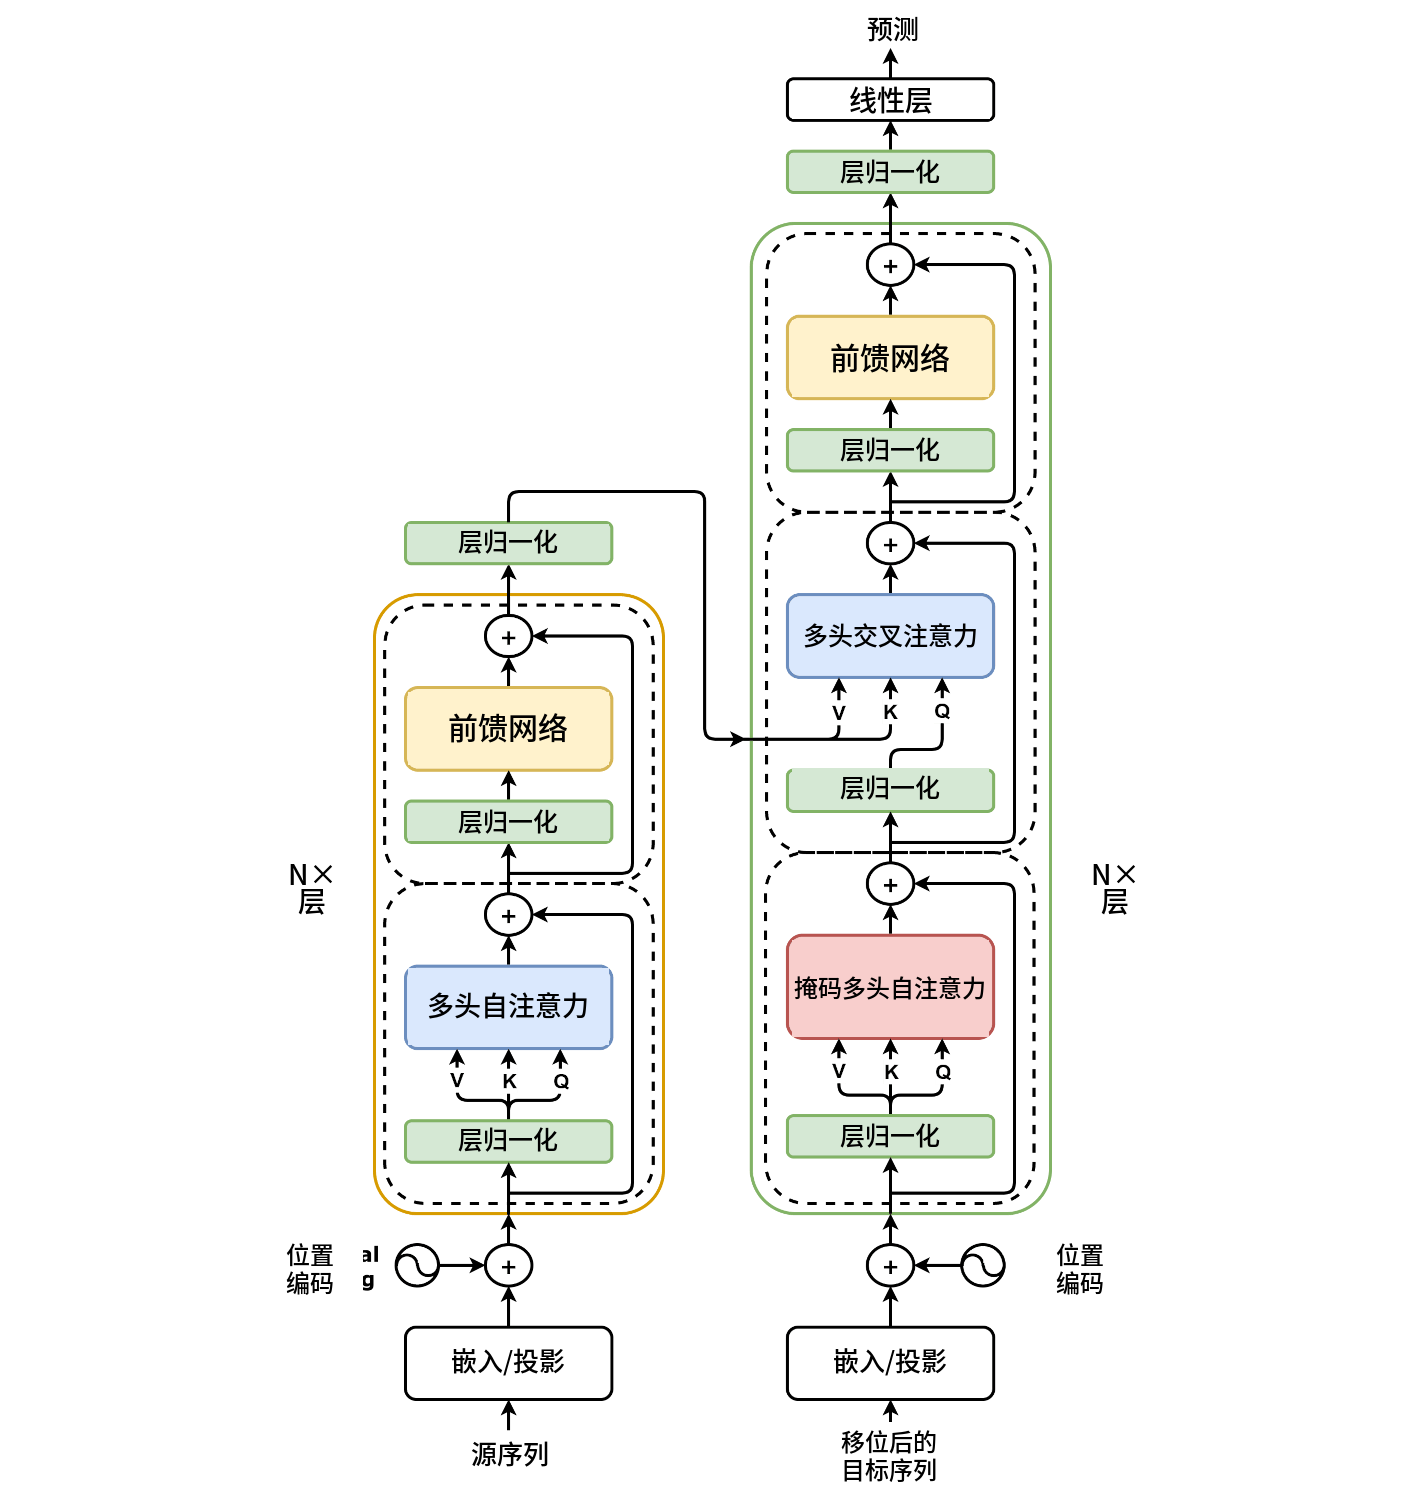
\includegraphics[width=0.7\linewidth]{part1/visuals/transformer_full_architecture.png}
    \caption{Transformer 架构示意 \citep{godoy_dl_visuals,vaswani2017attention}}
    \label{fig:transformer}
\end{figure}

下面我们更仔细地看看 Transformer 架构（请对照图示）。完整的架构由三类主要元素组成：嵌入、Transformer 块与输出概率：
\begin{enumerate}
\item 嵌入：首先，输入文本被分词，并投影为低维嵌入向量。嵌入上会加上位置编码，以保留词序。
\item Transformer 块：Transformer 块是该架构的主要特征。大多数模型由多层 Transformer 块构成。在每一层中，每个块包含三个元素：
\begin{itemize}
    \item 自注意力机制：注意力机制使词元之间能够建立长距离连接，捕捉词元之间的上下文信息与关系。多个注意力头让模型可以从不同角度考虑这些关系，例如用于短距离的句法联系，以及更宏观的语义语境。
    
    对于编码器堆栈，Transformer 使用自注意力；对于解码器堆栈，则使用掩码自注意力，以防「看到未来」。  
    \item 多层感知机：一个全连接的前馈网络独立地作用于每个词元。注意力层建立词元之间的联系，而多层感知机则可以精修每个词元的表示。
    \item 归一化：在大多数 Transformer 块中，都会加入归一化、正则化（dropout）与残差连接等典型深度学习方法，以防止梯度消失或爆炸，并使训练更稳定。     \end{itemize}
\item 输出概率：线性层与 softmax 层把处理后的嵌入转换为概率，用于做出下一个词元的预测。
\end{enumerate}
与 RNN、LSTM 网络等早期方法相比，Transformer 架构有两大优势。 %Transformers allow parallel processing of token sequence, unlike RNN, which must be processed in sequence. Furthermore, the attention mechanism enables long range context semantic relations to be recognized, preventing the model from forgetting early information, which is a problem with RNNs.
%These advantages of transformers, and the availability of large training corpuses, have enabled the successful development  of LLMs. 
基于注意力的 Transformer 支持（1）大规模并行处理，以及（2）细粒度的长距离语义连接——兼顾速度{\em 与}语义准确性。

自问世以来，Transformer 一直主导着语言建模。在大规模高质量训练语料建成之后，基于 Transformer 的大语言模型在问答、数据到文本生成以及应用驱动型任务上都取得了令人瞩目的表现。研究者们一直在追求越来越大的模型，并期待更强的能力 \citep{brown2020language}。在第~\ref{chap:scaling} 章中，我们将讨论如何进一步扩大性能。
%Powered by a large amount of language data and compute, large language models  have yielded strong empirical results across many fundamental language tasks such as   yet some specialized smaller models have appeared that outperform larger counterparts on various benchmarks. 


Transformer 架构是一个复杂的架构。网上有优秀的交互式教程提供了更多细节，\footnote{例如可参见 \url{https://poloclub.github.io/transformer-explainer/}}另见第~\ref{ch:nanochat} 章中的案例研究。


\begin{comment}
%Finally, we turn back to the input. 
The transformer architecture  eliminated the recurrent connections, we now process entire sequences in one go through a fully connected setup. However, in doing so, we lose the influence of sequential input. In other words, we can now present the input in any order, and the subsequent contextualized embedding will be the same. To fix this problem, we include a {\em positional encoding} for each token. This positional encoding embeds the absolute position of tokens. The original transformer paper \citep{vaswani2017attention} used a clever mathematical trick involving sine and cosine functions of different frequencies to create Rotary positional embeddings (RoPE), as in Equation~\ref{eq:pos-enc}, where $pos$ is the index of the token in the sequence, $i$ is the dimension index within the vector, and $d_{model}$ is the total size of the embedding vector. A visualization is given in Figure~\ref{fig:pos-emb}. While learned embeddings seem ideal, as they can fit any positional pattern, they are sensitive to the lengths observed during training. RoPE is fixed and structured, encoding position as rotation frequency, and works well irrespective of sequence length. 

\begin{align}
    \label{eq:pos-enc}
    PE_{(pos,2i)}               &=\sin(pos/10000^{2i/d_{model}})\\
    \nonumber PE_{(pos,2i+1)}   &=\cos(pos/10000^{2i/d_{model}})
\end{align}

\begin{figure}[t]
    \centering
    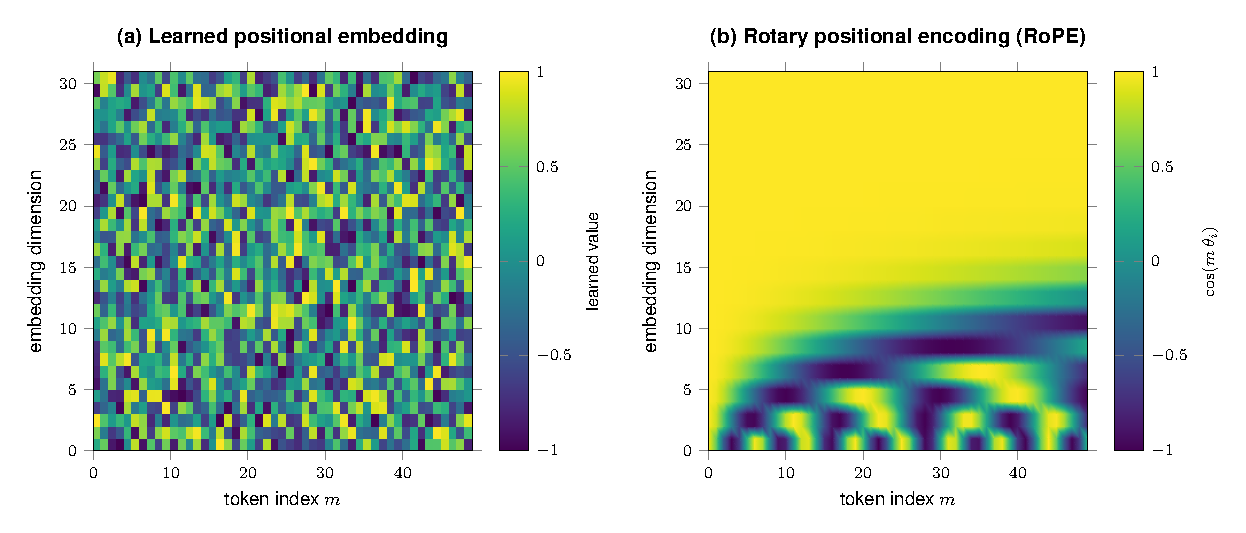
\includegraphics[width=.95\linewidth]{part1/visuals/positional_encodings.pdf}
    \caption{A visual contrast between arbitrarily learned positional embeddings, and fixed, structured rotational positional embeddings.}
    \label{fig:pos-emb}
\end{figure}
\end{comment}
    
\subsection{仅编码器（BERT）}
原始的 Transformer 模型是一个编码器—解码器组合结构，而现代模型通常要么是编码器、要么是解码器，因为人们发现两者各有其特定的实证优势。

下面我们更仔细地看看编码器。
编码器被训练用来把输入数据压缩成有意义的表示（嵌入），所用技术包括掩码语言建模（MLM）等。
它们擅长文本分类、情感分析这类自然语言理解任务；而解码器擅长文本生成、改写与摘要这类自然语言生成任务。

仅编码器模型的设计目标是产生输入文本的高质量向量表示（嵌入）。解码器是{\em 因果的}（只能看过去的词），而编码器与之不同，本质上是双向的：在编码器中，序列里的每个词元都可以同时关注其他所有词元。这种全局语境使模型能够为输入构建复杂的语义表示。
为训练这类模型，我们使用掩码语言建模。在这一过程中，大约 15\% 的输入词元会被替换为一个特殊的 \texttt{[MASK]} 词元。模型要自己学会：应当用词表中的哪个词元来填补这个位置。通常使用常规的交叉熵损失来更新模型。MLM 编码器训练的目标，是让模型利用周围的语境（左右两侧）来预测被掩码的词是什么。最终，这会迫使模型学会语法、语义，乃至一些世界常识。

为了提升学习效果，除 \texttt{[MASK]} 之外，编码器训练通常还会引入几个特殊词元：
\begin{itemize}
    \item \texttt{[CLS]}（分类）：插在最开头。经过所有层之后，该词元的最终状态被用作整个序列的聚合表示。
    \item \texttt{[SEP]}（分隔）：用来告诉模型一句话在哪里结束、另一句在哪里开始，这对问答等任务至关重要。
    \item \texttt{[PAD]}（填充）：确保一个训练批次中的所有序列长度相同。
\end{itemize}
最著名的仅编码器模型或许当属{\em 基于 Transformer 的双向编码器表示}，即更广为人知的 BERT~\citep{devlin2018bert}。
BERT 这类仅编码器模型，以及其后续的 RoBERTa \citep{liu2019roberta} 与 ALBERT~\citep{lan2019albert}，都已广受欢迎。

仅编码器模型非常适合迁移学习：它们先把输入嵌入，再针对下游任务（如某些应用领域的分类）进行微调。
%Encoder-only models often make use of \textit{bidirectional} or global attention, since we know the entire input at prediction time. 
构建仅编码器模型的流水线包含两个阶段：
\begin{enumerate}
    \item 预训练：先在一个包含数十亿词的大规模语料上训练模型。例如，它可能会学到 \textit{King} 与 \textit{Man} 相关、\textit{Queen} 与 \textit{Woman} 相关。此时模型还不知道如何做某件具体的事，它只是在学英语。预训练是一个昂贵的步骤，可能需要很长时间（数周或数月）。
    \item 微调：接着，取来预训练好的模型，在顶部加一个小的额外分类层（通常称为\textit{分类头}）。然后，用任务特定数据（如垃圾邮件检测或情感分析）把整个模型再训练一遍。由于模型已经理解语言，它通常只需要几千个样本就能成为新任务的专家。微调是一个廉价的步骤，可能只需几小时甚至几分钟；而如果从零开始做这项特定任务，则需要大规模数据集和大量训练时间。
\end{enumerate}
在讨论了仅编码器模型之后，我们接下来转向仅解码器模型。

\subsection{仅解码器（GPT）}
在语言生成任务中，使用的是仅解码器模型。
解码器通过自回归训练来重建数据或生成序列——它们通常一次生成一个词元。这种自回归依赖关系——下一个词元取决于此前已生成的内容——是一种\textit{因果}注意力。我们不能用未来的词元来推出最佳预测。
在编码器中，一个词可以看到它右边的词；而在解码器中，这是被严格禁止的。我们使用一个前瞻掩码（通常是一个三角矩阵），把未来词元的注意力得分设为 $-\infty$。如果模型要预测短语 \textit{The boy ate the...} 中的 \textit{apple} 一词，那么在训练数据中就不应允许它看到 \textit{apple} 这个词。解码器必须只依赖前文语境。因此，编码器使用掩码语言建模，而解码器使用（常规的）\textit{因果语言建模}，如下一章式~\ref{eq:lm} 所示。



因此，从编码器转向解码器时，预训练与微调之间的关系会略有变化：解码器在预训练中学的是预测下一个词，然后用同样的损失函数、但换一类数据来微调。这使我们得以走向{\em 上下文学习}（ICL）或提示学习：由于解码器被训练来续写序列，你只需给它一个提示词（即上下文），它就会生成答案，而无需任何权重更新。可以说，它是从提示词中的示例里学习 \citep{brown2020language}。大型解码器通过上下文学习即可轻松使用、无需进行昂贵的任务特定训练或微调，这让 ICL 引起了广泛兴趣。

仅解码器模型，例如{\em 生成式预训练 Transformer}（GPT）系列 \citep{radford2018improving,radford2019language,brown2020language,ouyang2022training,achiam2023gpt}，已经相当成功，如今在我们的社会中被广泛使用。此外还有许多其他模型被开发出来，既有开源的也有闭源的。
%
我们讨论的这些训练机制合在一起，构成了现代大语言模型流水线的基础，我们将在第~\ref{chap:pipeline} 章中更详细地解释。



\section{结语}
在本章中，我们追溯了自然语言处理从语言学的根基到驱动当今大语言模型的神经架构这一非凡演进历程。我们论证了人类语言本身是复杂的，其特点在于句法、词法的繁复规则以及深层的语义与语用微妙之处。现代自然语言处理的突破经历了一系列范式转变——符号式、统计式、神经式——为当代语言模型提供了基本构件，而这些模型建立在稠密嵌入、注意力机制，以及数据、模型规模与算力上的规模化增长之上。编码器模型适合自然语言理解，解码器模型适合自然语言生成。两者都通过预训练与微调来训练，而解码器还支持基于提示词的上下文学习。  %Driven by robust machine learning paradigms, these training methodologies are what ultimately breathe functional life into the models.

\subsection{开放挑战}
尽管现代大语言模型的表现令人印象深刻，也存在许多有用的用例，但仍有重要挑战尚待解决。 %Many impressive inventions have progressed NLP from simple count-based systems to (Agentic) LLMs. However, as we push the boundaries of what machines can understand, several fundamental challenges mentioned so far are ever prevalent. 
理解这些挑战，对于识别研究空白、构建更稳健的系统都至关重要，这对智能体式大语言模型同样适用。

\paragraph{性能规模化}
当前的语言建模以{\em 缩放定律}（scaling law）为前提：更多的参数、更多的数据与更多的算力这三者共同带来更好的泛化。然而，进一步扩大规模会带来显著挑战。要达到最先进的性能，可能需要拥有数十亿参数的模型，其训练在算力上耗费数百万美元，环境代价高昂。如何用高效的架构实现更好的泛化（即完成模型未被训练过的任务的能力），仍是一个开放问题。当前研究正在探索模型剪枝与量化（两者都在第~\ref{chap:scaling} 章讨论）。此外，合成数据生成（见第~\ref{chap:synthetic-data} 章）旨在不增加训练数据的前提下获得更高的泛化能力，但模型规模与泛化能力之间的最佳平衡点依然难以捉摸。

\paragraph{数据稀缺}
大多数自然语言处理训练数据集都是为英语构建的，主要基准也是如此，例如 GLUE（通用语言理解 \citep{wang2018glue}）或 SQuAD（问答 \citep{rajpurkar2016squad}）。这些数据往往来自大规模的网页抓取。其他高资源语言（如中文或印地语）也能从这种做法中受益，而低资源语言（如荷兰语或佛兰芒语）则缺乏从零训练现代 Transformer 所必需的数字化足迹与文化存在感。由于模型会继承其训练数据的文化细微之处，非英语使用者常常遭遇性能下降，或遭遇偏向西方视角与语言规范的算法偏见。

\paragraph{多语言性}
由于可用资源存在差异，自然语言处理很少能为每种语言都提供通用方案。例如，把一个模型在英语上的成功迁移到其他语言，会引入若干语言学上的复杂性。
土耳其语、芬兰语或阿拉伯语等语言在形态上可能更丰富，它们通过动词或名词的前缀与后缀传递大量信息。土耳其语中的一个词可能对应英语中的一整句话。未在此类语言上训练过的模型，无法体现这种语言上的丰富性。  

此外，不同语言可能使用不同的字符集与书写系统。这给处理非拉丁文字带来问题（例如中文的表意文字，或希伯来语与阿拉伯语的辅音音素文字）。这些语言需要新的分词与嵌入策略，才能得到合理的子词。

\paragraph{语言演变}
语言是活的，其演化速度快于模型重新训练的速度。这尤其会导致未登录词（OOV）问题。即便有了子词分词（如字节对编码（BPE）\citep{gage1994new} 或 WordPiece \citep{song2021fast}），模型仍难以应对新造词、俚语、技术行话，或训练截止时尚未存在的名称。此外，一个在 2022 年训练的模型，可能无法理解 2026 年全球事件或文化变迁的语境（比如「Z 世代的凝视」是什么？）。创建一种既能更新知识、又不会遗忘先前信息（灾难性遗忘）的持续学习系统，仍是一个开放挑战 \citep{wu2024continual}。

\paragraph{超越文本的分词}
随着人们努力去理解传统语境之外的信息，文本与其他模态之间的界限正在模糊。为此提供语境的一个挑战是多模态表示：把图像、音频与视频表示在与文本相同的潜空间中。文本是离散的（词／字符），而音频与视频是连续信号，必须经过采样与量化。要把一帧视频或一段波形映射为语言模型能够与文本一同处理的词元，需要 Vision Transformer（ViT）\citep{han2022survey} 或对比语言—图像预训练（CLIP）\citep{radford2021learning} 这类复杂架构。第~\ref{chap:world} 章将讨论多模态模型。

\paragraph{可解释性}
最后，一个重要开放问题是这些模型内部如何运作。我们能够衡量一个模型是否有效，却往往难以解释它为何给出某个特定答案。此外，模型经常出错或产生幻觉，以令人信服的方式给出错误答案。对于军事、法律或医疗等高风险自然语言处理应用而言，缺乏透明度应当成为采用语言模型的重大障碍。可解释语言模型的技术，例如机制可解释性，将在第~\ref{chap:mi} 章讨论。

除上述挑战之外，语言建模还面临许多其他社会技术层面的挑战，包括伦理对齐、长篇逻辑推理等。随着自然语言处理持续演进，这些开放问题构成了一片动态的前沿：解决其中一个挑战，往往又为下一代的学子、研究者与工程师揭示出一系列更深层的问题。

\subsection{展望}
在本章中，我们讨论了语言建模的基础知识，从早期起源到现代解码器模型。现在，我们已准备好更深入地探讨智能体式大语言模型这一主题。在下一章中，我们将更详细地讨论一个大语言模型的训练流水线是如何运作的。

\bibliographystyle{plainnat}
\bibliography{agenticbook,refs,case,synthetic}


% \begin{comment}
% \section{Training Paradigm: Supervised Learning. Why?}
% static dataset (in distribution) of labeled examples, learn regression or classification on the static dataset in order to predict out of distribution.

% Sample many epochs over the examples in the dataset to fit the parameters defining the curves/classes.

% Learning is conceptually quite simple: just variables for the parameters, a min operator (which is a simple conditional statement) to minimize the loss between the predicted label and the real label, and a while-loop to keep on iterating until we have converged enough (the sum of the error does not change much between training epochs).

% \section{Training Paradigm: Reinforcement Learning (Aske). Why?}
% \subsection{Offline and Online Learning}
% Supervised and Reinforcement. Stable and Unstable.

% Interactive learning is algorithmically exactly as simple as offline learning: a while loop around a max operation that improves the reward of the action for each state of the policy. The only difference is that there is no static dataset, but data items are chosen by using the current policy to take an action to create a new state, and getting the label, the reward, for that state/action combination, from an environment. The environment is like an oracle that plays the role of the dataset. 

% \subsubsection{Exploration}
% There is a complication in that the next state is determined online, dynamically, and the algorithm can get stuck in a feedback loop (converge on a local optimum), or have bad coverage of the state space (converge on a local optimum). Special measures have to be taken to make reinforcement learning well behaved, that are not needed in supervised learning. Reinforcement learning algorithms must explore. 

% \subsubsection{Credit assignment}\label{sec:sdp}
% Furthermore, reinforcement learning typically allows a general setting in which not all states have a reward defined. Also, the concept of state and action imply that states are connected: a policy is also a path, a trajectory, a trace, an episode, of timesteps through the state space. The policy is interpreted not as a curve or a classification, but as a function that defines the optimal actions from a start state, that finds the optimal expected cumulative future reward. In supervised learning the examples in the dataset are independent. There is no causal connection between two pictures of dogs. It is a dataset of independent singular decision problems.  In reinforcement the states are causally connected by the actions, the reinforcement learning problem (MDP) defines a sequential decision problem. Each state is a time step in the system towards a final state. The policy is the optimal solution for the sequential decision problem, giving the actions, for each state, that find the best reward of a path/episode/trace/trajectory.

% Reinforcement learning algorithms, such as Q learning, solve the credit assignment problem, which is how to take an action in the present that takes into account the rewards of future states. 

% Interestingly, the algorithm is the same: just a while loop that maximizes.

% \subsubsection{Loss and Reward}
% Note that in supervised learning we minimize (loss) and in reinforcement learning we maximize (reward). Very confusing. Just keep in mind that in supervised learning a loss is minimized, and in reinforcement learning a reward is maximized.

% \subsubsection{Operational Considerations}
% Machine learning started with supervised learning, where a dataset must be present for the algorithm to work. After the instability issues of reinforcement learning were solved, reinforcement learning has become quite popular. It is quicker to use, online, as soon as one reward is available, an optimization pass can be done, no need to first collect a full dataset of examples. RL is also able to solve open ended problems, online, it learns as it goes, it optimizes running processes where that training data is incomplete. 

% Note that this ease of use advantage does not fully remove the dangers of local optima: in open ended problems there is always the danger that RL only partially covers the state space, remains stuck in a friendly part of the state space, or even in feedback loop. A typical way to prevent this problem is to run the algorithm for a long time, to reduce learning rates, or to increase exploration of random moves, not taking advantage of existing policies. For open ended problems RL algorithms can be quite slow.

% \subsection{Interaction: Agent/Environment}
% %\subsection{Optimal Reward Policy}
% %\subsection{Tabular and Deep Algorithms: Q-learning, DQN, PPO}
% \subsubsection{Markov Decision Process}
% Grid world example
% \paragraph{State}
% Language

% Vision

% Action

% \paragraph{Action---Agent}
% \paragraph{Transition---Environment}
% \paragraph{Reward---Environment}
% \paragraph{Policy---An action for each state}


% \begin{figure}[t]
%   \begin{center}
%     \input figures/rl
%     \caption{Reinforcement Learning}\label{fig:rl-org}
%   \end{center}
% \end{figure}
% Figure~\ref{fig:rl-org} illustrates how a reinforcement learning agent learns a policy with an action for each state, online, through interaction with the environment.


% \paragraph{RL Intuition}
% \begin{itemize}
%     \item[Credit Convergence]
% Bellman equation, Sampling/Target network/Replay Buffer
% %\subsubsection{Unknown Transition Function}
% Monte Carlo Sampling
% \item[High Variance]
% Bootstrapping:  Temporal Difference Learning, Region methods
% \item[Exploration]
% Epsilon Greedy, Entropy methods
% \item[Off-policy learning]
% Q-learning
% \item[Continuous Actions]
% Direct Policy-based Methods REINFORCE
% \item[High Dimensional State Representation]
% Deep learning Representation, JAX
% \item[Tabula Rasa: Curriculum Learning Beyond Dataset]
% AlphaZero

% Metalearning, transfer learning

% \end{itemize}

% Matrix for DP, MC, SARSA, Qlearning, DQN, PQN, REINFORCE, TRPO, PPO, TD3, SAC and the challenges that they solve


% \subsection{RL for LLM Training}
% See: \citep{liu2025part}
% \subsubsection{RLHF}
% \subsubsection{DPO}
% \subsubsection{GRPO}
% \end{comment}
